\documentclass[10pt]{jsbook}

\usepackage[ipaex]{pxchfon}
\usepackage[top=20truemm,bottom=20truemm,left=35truemm,right=35truemm]{geometry}
\usepackage{titlesec}
\usepackage{picture}
\usepackage{graphicx}
\usepackage{listings,jlisting}

\usepackage[usenames]{color}

% 四角枠
\usepackage{ascmac}

% URL
\usepackage{url}

\usepackage{amsmath,amssymb}

% colors
\definecolor{teal}{RGB}{0,128,128}
\definecolor{powderblue}{RGB}{176,224,230}
\definecolor{darkslateblue}{RGB}{72,61,139}
\definecolor{darkslategray}{RGB}{47,79,79}
\definecolor{lightcyan}{RGB}{224,255,255}
\definecolor{deepblue}{rgb}{0,0,0.5}
\definecolor{deepred}{rgb}{0.6,0,0}
\definecolor{deepgreen}{rgb}{0,0.5,0}

% 太さ
\DeclareFixedFont{\ttb}{T1}{txtt}{bx}{n}{12} % for bold
\DeclareFixedFont{\ttm}{T1}{txtt}{m}{n}{12}  % for normal

% chapter                                                                             
\titleformat{\chapter}[block]
{}{}{0pt}{
	\fontsize{40pt}{40pt}\selectfont\filleft
}[
\hrule \Large{\filleft 第 \thechapter 章}
]

% section
\titleformat{\section}[block]
{}{}{0pt}
{
	\hspace{0pt}
	\normalfont \LARGE\bfseries \thesection
%	\normalfont \Huge\bfseries \thesection
	\hspace{0pt}
}
[
\begin{picture}(100,0)
%\put(3,30){\color{teal}\line(1,0){400}}
\put(3,18){\color{teal}\line(1,0){350}}
\end{picture}
\\
\vspace{-50pt}
]

% subsection
\titleformat{\subsection}[block]
{}{}{0pt}
{
	\hspace{0pt}
	\normalfont \Large\bfseries \thesubsection
	\hspace{0pt}
}
[
\begin{picture}(100,0)
\put(3,18){\color{darkslateblue}\line(1,0){300}}
\end{picture}
\\
\vspace{-30pt}
]

% margin
\addtolength{\textwidth}{0in}
\addtolength{\oddsidemargin}{0in}
\addtolength{\textheight}{0in}
\addtolength{\voffset}{0in}
%\parindent=0zw


% 演習
\newtheorem{practice}{演習}[section]

% Python
% Python style for highlighting
\newcommand\pythonstyle{\lstset{
language=Python,
basicstyle=\ttm,
otherkeywords={self},             % Add keywords here
keywordstyle=\ttm\color{deepblue},
emph={MyClass,__init__},          % Custom highlighting
emphstyle=\ttm\color{deepred},    % Custom highlighting style
stringstyle=\color{deepgreen},
frame=tb,                         % Any extra options here
showstringspaces=false            % 
}}


% Python environment
\lstnewenvironment{python}[1][]
{
\pythonstyle
\lstset{#1}
}
{}

% Python for external files
\newcommand\pythonexternal[2][]{{
\pythonstyle
\lstinputlisting[#1]{#2}}}

% Python for inline
\newcommand\pythoninline[1]{{\pythonstyle\lstinline!#1!}}


%opening


\begin{document}

% イントロダクション
\chapter{Intro}
%!TEX root = ../main.tex
\section{Deep Neural Networksの基礎}
\subsection{なぜいまAIブームなのか}
現在、第3期AIブームだといわれる。第1期は1956年に開催されたダートマス会議を契機として1970年前半まで続いたもので、パーセプトロンの原理が発明され、数学定理の証明や言語意味理解などが試みられた。第2期は1980年台に起こり、Multi Layer Perceptron (MLP)を効率よく学習させるBack Probagation (BP)手法が確立されたほか、ある専門領域の知識を何らかの形で抽出し質問に答えたり問題を解いたりするエキスパートシステム研究が盛んに行われた。国内でも第五世代コンピュータの研究開発プロジェクトに莫大な資金が投入された。しかし、いずれのブームも大きな失望感とともに急速に廃れ、とある国際会議ではArtificial Intelligenceというキーワードが入っているだけで論文が落とされるというジョークもまことしやかにささやかれるほどであった。

では、いまなぜ改めて第3期AIブームなのだろうか?現在のAIブームを牽引しているのはDeep Neural Networks (DNN, 深層学習)であることは間違いない。しかし、現在のDNNの源流となるネオコグニトロンは1980年前後にすでに(当時NHK放送技術研究所の)福島ら\cite{fukushima79,fukushima80,fukushima83}によって提案されている。原因は諸説あるが、下記のような複数の技術的要因がうまく噛み合ったためだと思わる。
\begin{itemize}
\item SNSの流行、IoT技術の普及などにより様々なドメインのデータがビッグデータ化した。
\item GPUやクラウドコンピュータなどDNNを現実的な時間内で計算終了できるだけの計算資源が得られるようになった。
\item クラウドワーキングによって正解データを作成してくれる人の確保が格段に容易になった。
\end{itemize}
特にDNNをうまく動作させようと思うと、学習のための膨大なデータが必要である。Weakly-supervised Learning (弱教師学習)やSemi-supervised Learning (半教師付き学習)など全てのトレーニングデータに正解を付与しなくともある程度学習ができるようになるアルゴリズムは存在するが、それは正解が得られない場合の回避策であり、全てのトレーニングデータに対して正解が付与されている状態が最大の性能を発揮する。半導体の講義で学習したであろうムーアの法則に則って考えると、計算機は3年で4倍の性能を得ることができるので30年前と比べてざっと100万倍の計算能力を手に入れた計算になる。これは、現在1日かけて行う計算は30年前の計算機では100万日かかっていたことを意味するが、30年前から今日まで1万日ちょっとしか経っていない。

さらには、社会的な情勢もそれを後押ししたと指摘する研究者もいる。
\begin{itemize}
\item Google, Facebook, Microsoftなど巨大IT企業がDNNを重要視し、それぞれTensorFlow, PyTorch, The Microsoft Cognitive Toolkit (CNTK)などのディープラーニングフレームワーク(ソフトウェアライブラリ)を作成・公開した。また、国内でもPFN社がChainerを公開。
\item オープンソース化が主流となり、GitHubなど多くのプラットフォームを利用して団体や個人が作成したソフトウェアが公開去れるようになった。これにより、自分で実装をする必要がなくなり、すぐに試せる、もしくは公開されている機能から先のみを実装すればよくなった。
\item 論文もオープンソース化の流れにのり、多くの出版社でオープンソースとして公開去れることが増えた。また、ArXivのように速報性を重視するサービスも登場し、その流れを一層加速させた。
\item 物体認識コンテストのように、多くのコンテストが開催され、同じデータで多くの研究者が競い、性能の差異が議論しやすくなった。また、Kaggleのようにコンテスト・ランキングをビジネスにするサービスも現れた。
\end{itemize}
学生の諸君は信じられないであろうが、ほんの10-20年前は画像を読み込むにも自前で実装するところから始めなくてはならなかった。そのため、ソフトウェアの開発効率は今と比べて極めて悪かったのである。いまはArXivにいち早く一流国際会議に投稿された会議が掲載され(当落の保証はない)、ソースコードとデータセットが同時に公開され、それらをDLすれば一瞬で再現でき、しかも前述のフレームワークの登場で可読性が極めて高く改変がやりやすい。という時代である。Twitterやブログで一気に話題化するのも要因の一つであろう。



\subsection{人工知能, 機械学習, 深層学習}
人工知能, 機械学習, 深層学習が同列に語られることも多いが、厳密に言うと機械学習は人工知能技術の1つであり、深層学習は機械学習技術の1手法という位置づけである。特にマスコミの記事などでは受けの良さから「人工知能による処理」と謳うものが多くなりがちであるが、必ずしもそれは学習ベースの処理出ないこともあるので注意が必要である。

\begin{figure}[ht]
	\begin{center}
		\includegraphics[width=0.7\linewidth] {images/YamasakiLab/introduction/AI_ML_DNN.eps}
		\caption{人工知能、機械学習、深層学習の関係。}
		\label{fig:accuracy}
	\end{center}
\end{figure}


\subsection{DNNは何が破壊的だったか?}
画像認識を例に、果物の画像を分類するシステムを開発すると仮定しよう。りんごとみかんとバナナ・・・を認識しようとしたとき、自分でプログラムを書くとしたら何を手がかりとしてそれらの画像を分類するだろうか?赤ければりんご、橙色であればみかん、黄色であればバナナ・・・としてみればどうだろう。しかし、これは例えば青りんごや未完熟の緑色の果実はうまく分類することができない。それでは、大きな丸い形はりんご、小さい楕円形はみかん、長細ければバナナ・・・としてみてはどうだろう。と、このように複数のクラスをうまく切り分けることのできる画像特徴を考えるのが一般的である。DNN以前の画像認識はまさにこの例に述べた通り画像認識に有効な新しい特徴を人間が考えるというのが画像認識の研究だった。特徴ベクトルを一旦抽出することができればあとはSuport Vector Machine (SVM)やRandom Forest (RF)など成熟した既存の機械学習器を用いて実際の認識・分類を行う。

DNNを用いた画像認識では、DNNに与えるのは画像そのものと正解ラベルのみである。画像を分類するための特徴はDNNが自動で考えるのである。言葉で記述するとそれだけなのであるが、人間が特徴を考えるよりも効率的な特徴設計ができる。画像分類ではILSVRCという1000クラスの画像を分類する国際コンテストが行われている。DNN以前は何らかの工夫により毎年1~2\%ずつ誤差率が下がっていくというのが一般的であったが、2012年にDNNが初めて用いられたときには人間が考えた特徴量による最高性能が誤差率26\%であったのに対し、DNNの誤差率は15\%と、実に10\%以上もの差をつけて大勝した。その後、DNNは音声やタンパク質の結合予測コンテストでも軒並みこれまでの「人間が考える特徴量」に大差をつけて優勝し、DNN大流行のきっかけとなった。

もちろん、DNNの登場によってやることはなくなったかというとそうではない。DNNは深層学習の一般的な呼称であり、どのようなネットワークを構築するかは利用者の手に委ねられている。また、学習に関わる様々なハイパーパラメータなども人間が決定しなければならない。

\begin{figure}[ht]
	\begin{center}
		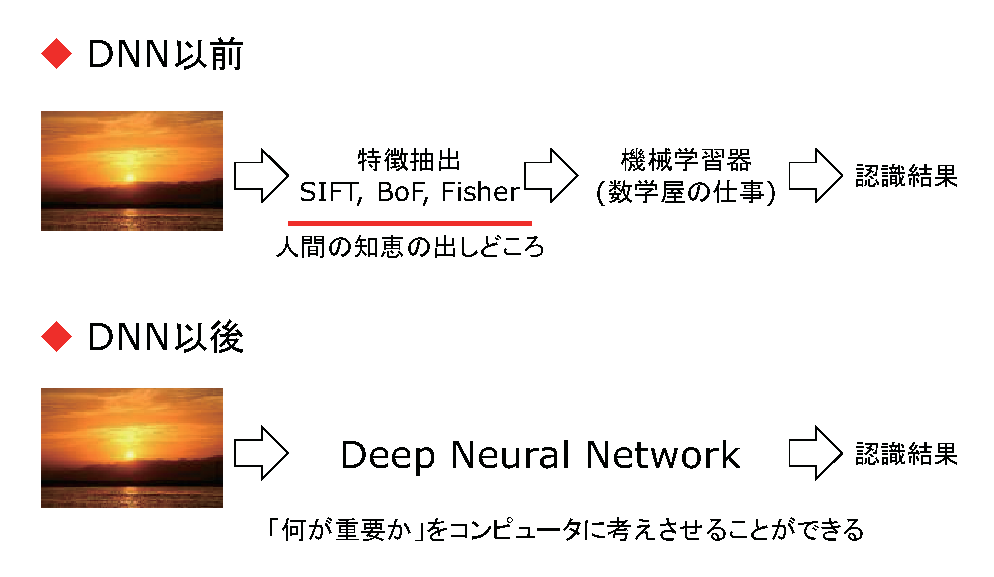
\includegraphics[width=0.7\linewidth] {images/YamasakiLab/introduction/before_after_dnn.eps}
		\caption{DNN以前とDNN以後の画像認識手法の違い。}
		\label{fig:accuracy}
	\end{center}
\end{figure}

\subsection{DNNの特徴}
上記に述べた通り、特徴の設計も自動的にできるという利点以外に、下記にあげるような利点・特徴がある。

\subsubsection{バッチ型ではなく逐次型の学習である}
Support Vector Machine (SVM), Random Forest (RF)を始め、主要な機械学習技術の殆どがバッチ型学習、すなわち学習データはすべてそろえたあとすべてを一気に使って学習させるという手法をとる。そのほうが学習データの分布を見渡した上で最適な学習が行えるためである。SVMやRFを逐次学習、すなわち少しずつ学習データが増えていった場合に対応去せる試みもなされてきたがバッチ学習と比べると精度は遠く及ばないものであった。

それに対して、NNは学習データを少量ずつ見ては内部のパラメータを更新していくという手法をとる。もちろん、初期のパーセプトロンでは学習データ1つごとにパラメータ更新を行っていたが、それではBPを行った際ノイズに弱くなるので現在のDNNでは複数の学習データに対する誤差を平均化してBPする手法(ミニバッチ)など工夫はなされている。逐次学習は裏を返せば学習を途中で止めて、その後ネットワーク構造や学習データを変化させて学習を続けても良いということを示しており、この特徴が下記に続く様々な特徴へと続いていく。


\subsubsection{Transfer learning (転移学習)が容易である}
対象とするクラスの教師画像が多数無い場合が存在する。最初大量にトレーニング画像を準備できるクラスでpre-trainしたあと対象クラス画像でfine-tuneすると高性能が出ることが知られている。例えて言えば、果物の分類器と花の分類器があったとする。果物の画像は集めるのが容易だが花の画像を集めるのは困難であるとしよう。これまでは、果物の分類器と花の分類器は独立して学習しなければならず、果物の分類器を花の分類に転用するのは困難な問題であった。そのため、花の分類性能を向上させるためには花のトレーニングデータの数を増やすしかなかった。

しかし、DNNでは
\begin{itemize}
\item ある程度画像認識一般に有用な汎用的な特徴表現を内部表現として獲得している
\item 逐次学習であるため、途中からトレーニングデータを変えても学習を進められる
\end{itemize}
などの特徴があるためである。この特徴のお陰で様々な分野へ画像分類の応用が可能となった。ただし、闇雲にデータを集めても転移学習がうまくいくわけでなく、画像の種類が大きく異なるような場合は転移学習の効果が得られにくくスクラッチ学習(他のデータを使わないで0から学習)したほうが性能が高い場合もあるので注意が必要である。また、そのような問題に対して研究するCross-Domain Learning (ドメインを跨ぐ学習)という研究領域も存在する。



\subsubsection{ネットワークの分岐が容易である}
Neural Networkは文字通りネットワークであるため、途中で分岐させることが容易である。これが、DNNの性能を向上させる要因の一つとなっている。

\subsubsubsection{ネットワークが途中で複数に分離する場合}
途中までのネットワーク構造を共通にして、途中から複数に分離し、複数のタスクを解くネットワークを学習させることができる。これをMulti-task Learningと呼ぶ。前段の共通ネットワークは、複数のタスクからの誤差率が逆伝搬されパラメータがアップデートされる。すなわち、前段ネットワークは複数タスクを同時に解くのに効率的なネットワークになっていることが期待される。

\subsubsubsection{ネットワークが途中で1つに集約する場合}
複数のネットワークに異なるモーダルのデータを入力し、途中で1つのネットワークに統合してタスクを解くネットワークを学習させることができる。これをMulti-feature Fusionと呼ぶ。これまでの機械学習では、画像、音声、テキストなどモーダルの異なるデータを融合して総合的に学習を行うことが困難であった。しかし、このネットワーク構造では複数種類のデータをどのように結合すればよいかについてもDNNが自動的に最適化するので無理のないMulti-feature Fusionが可能となる。

\begin{figure}[ht]
	\begin{center}
		\includegraphics[width=0.7\linewidth] {images/YamasakiLab/introduction/branch.eps}
		\caption{ネットワークの分岐。(左) Multi-task Learning、(右) Multi-feature Fusion。}
		\label{fig:accuracy}
	\end{center}
\end{figure}

\subsubsection{データのモーダル間の垣根が少なくなった}
本実験ではたった10日間の日程で画像・音声・言語を対象としている。一昔まえであればそれぞれ10日間のプログラムにしてもおかしくないほど異なる専門知識が必要とされたきた。しかし、DNNによって画像・音声・言語といったモーダルの違いは以前に比べて意識しなくても良くなってきている。それぞれのモーダルに応じてちょっとした前処理に違いは生じるものの、一旦DNNの中に入力してしまえば、もしくはDNN特徴量として表現してしまえば、それらのデータの扱いは全く同じになる。それを証拠に、現在image2text, text2imageといった画像と言語の融合や、「猫」という画像表現と「猫」の鳴き声が特徴空間では互いに近くなるよう学習する手法などが登場している。

\subsection{Neural Network基礎}
山崎の講義を参照すること。




% 自然言語部分
\chapter{Natural Language Processing}



%\section{ニューラルネットワークを用いた自然言語処理}

本課題では,ニューラルネットワークを利用した自然言語処理の中核的な技術
である,sequence-to-sequence モデル(以下,seq2seqモデル)の基本的な原理と動作を学ぶ.
Seq2seq モデルは,単語列や文字列といった「系列」を入力し,新たな系列を出
力することのできるニューラルネットワークモデルであり,機械翻訳や質問応答,対話といっ
た様々な言語処理タスクへの応用が急速に進んでいる.なかでも機械翻訳に関しては,
近年の翻訳精度の向上に大きく貢献し,従来の統計的機械翻訳よりも格段に流暢な
翻訳を可能にしている \cite{wu2016google}.


%\subsection{単語ベクトル}
%
%Seq2seqモデルでは,単語を実数値のベクトルとして表現する.
%
%ニューラルネットワークを用いた自然言語処理では,単語を実数値のベクトルで表すことが多い.
%
%ベクトルの近さや cos類似度が単語の文法的・意味的な近さを表す.
%
%単語ベクトルの代表的な学習法を紹介する.
%
%
%\subsection{CBOWモデル}
%
%
%\subsection{Skip gram モデル}
%
%Skip gram モデル \cite{NIPS2013_5021} を説明する.

%\begin{equation}
%\frac{1}{T} \sum_{t=1}^T \sum_{-c \leq j \leq c, j \neq 0} \log p(w_{t+j} | w_t)
%\end{equation}
%
%$p(w_{t+j} | w_t)$ は以下のようにソフトマックス関数で定義される.
%%\begin{equation}
%p(w_O | w_I) = \frac{\exp({v'_{w_O}}^\top v_{w_I})}{ \sum_{w=1}^{W} \exp({v'_w}^\top v_{w_I})} 
%\end{equation}
%
%
%\subsection{実験課題}
%
%
%https://github.com/chainer/chainer/tree/master/examples/word2vec


\section{リカレントニューラルネットワーク}
\label{sec:rnn}

自然言語処理では,文字列や単語列といった「系列」を扱う処理が多い.しかし,通常のフィード
フォワードニューラルネットワークでは,入力と出力の次元数は固定されており,任意の
長さを持つ系列を扱う処理には適さない.
それに対して,
リカレントニューラルネットワーク (recurrent neural network, RNN) では,ネットワークに「状態」
を持たせることによって,任意の長さの系列を扱うことを可能にしている.


\begin{figure}[b]
 \begin{center}
  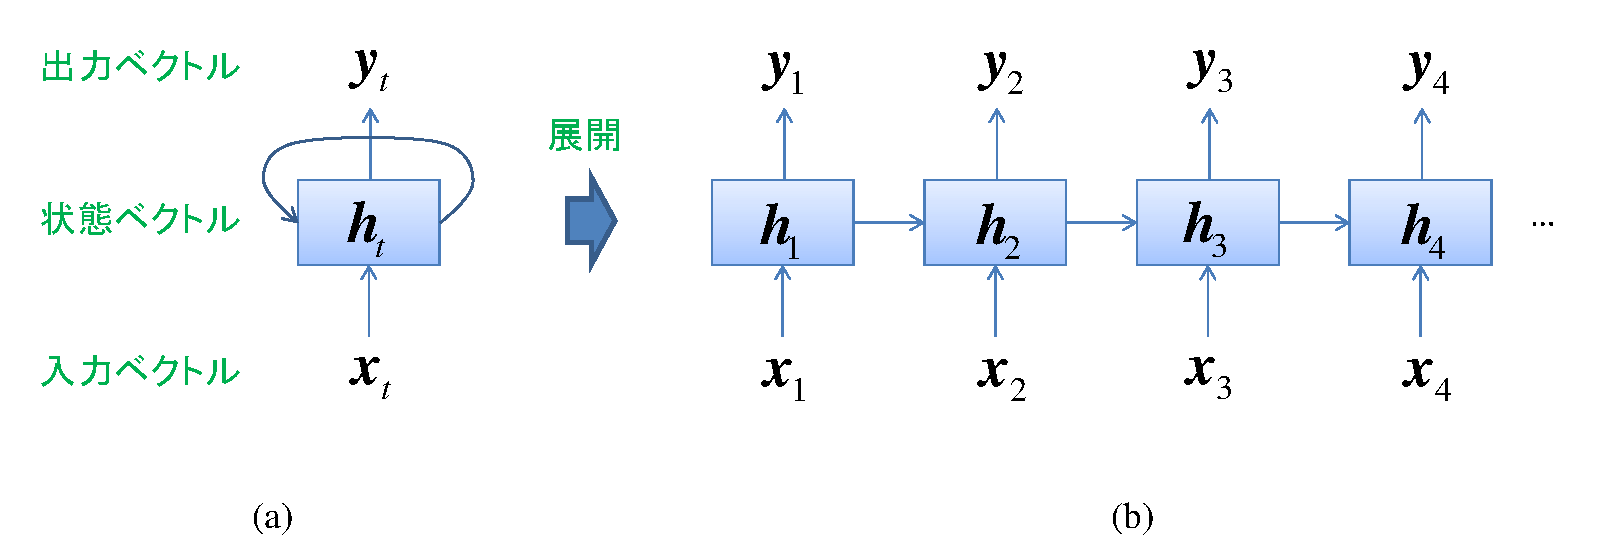
\includegraphics[width=140mm]{images/TsuruokaLab/rnn1.eps}
 \end{center}
 \caption{リカレントニューラルネットワーク}
 \label{fig:rnn1}
\end{figure}

図\ref{fig:rnn1}にリカレントニューラルネットワークの構造を示す.図\ref{fig:rnn1}(a)に示すように,
リカレントニューラルネットワークでは,ネットワーク自身が状態$\boldsymbol{h_t} \in \mathbb{R}^H$ を持つ
ことによって,その時点での入力$\boldsymbol{x}_t \in \mathbb{R}^D$ だけではなく,過去の入力
$\boldsymbol{x}_1,\boldsymbol{x}_2,...,\boldsymbol{x}_{t-1}$ にも
依存するような値$\boldsymbol{y_t} \in \mathbb{R}^V$ を出力することができる.
単純なリカレントニューラルネットワークでは,状態$\boldsymbol{h_t}$ は,
\begin{equation}
\boldsymbol{h_t} = \tanh(\boldsymbol{W}_h \boldsymbol{x}_{t} + \boldsymbol{U}_h \boldsymbol{h}_{t-1} + \boldsymbol{b}_h)
\end{equation}

\noindent
と計算される.ここで,$\boldsymbol{W}_h \in \mathbb{R}^{H \times D}$,$\boldsymbol{U}_h \in \mathbb{R}^{H \times H}$,
$\boldsymbol{b}_h \in \mathbb{R}^D$ は,このリカレントニューラルネットワークの動作を決めるパラメータである.

リカレントニューラルネットワークは,一見普通のフィードフォワードニューラルネットワークと大きく異なる
仕組みのように見えるが,実は本質的には通常のフィードフォワードニューラルネットワークと同じものである.
図\ref{fig:rnn1}(a)のリカレントニューラルネットワークを時間方向に展開して考えると,
図\ref{fig:rnn1}(b)に示すように,
パラメータ $\boldsymbol{W}_h$,$\boldsymbol{U}_h$,$\boldsymbol{b}_h$ を共有した多数のフィードフォワードネットワーク
を連結したものと等価であることがわかる.したがって,パラメータの学習も通常のフィードフォワードニューラルネットワーク同様,
誤差逆伝播法 (backpropagation) によって効率的に行うことができる.


\section{言語モデル}

\begin{figure}[t]
 \begin{center}
  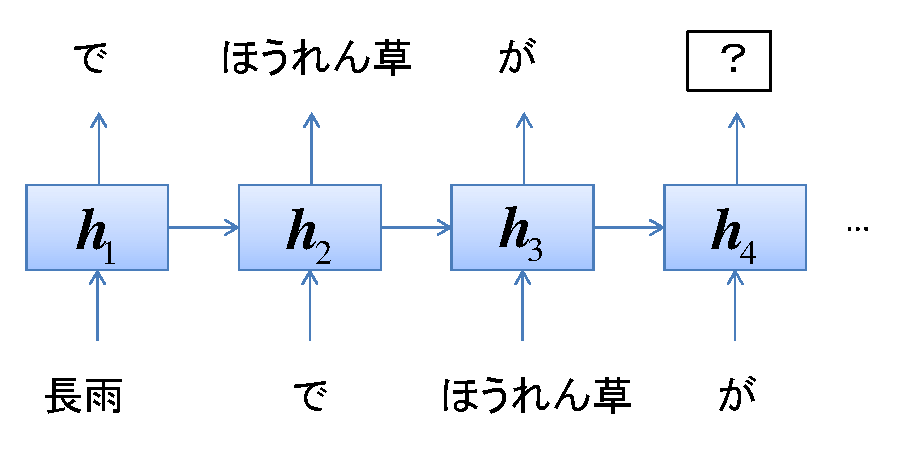
\includegraphics[width=80mm]{images/TsuruokaLab/lm.eps}
 \end{center}
 \caption{言語モデル}
 \label{fig:lm}
\end{figure}

リカレントニューラルネットワークを利用すると言語モデル(language model)を容易に実現することができる \cite{mikolov10lm}.
言語モデルでは,単語列$w_1,w_2,...,w_n$の生成を以下のような確率モデルで表現する.
\begin{equation}
P(w_1,w_2,...,w_n) = \prod_{t=1}^n P(w_t | w_1,...,w_{t-1})
\end{equation}

ここで図\ref{fig:lm}のように,リカレントニューラルネットワークの入力として,単語列$w_1,w_2,...,w_{t-1}$ 
% に対応するベクトルの列$\boldsymbol{x}_1,\boldsymbol{x}_2,...,\boldsymbol{x}_{t-1}$
を考え,出力として,単語列$w_2,w_3,...,w_{t}$
を考えれば,文脈$w_1,...,w_{t-1}$ から,次に出現するであろう単語$w_t$ を予測する
モデル $P(w_t | w_1,...,w_{t-1})$ が実現できることになる.$P(w_t | w_1,...,w_{t-1})$ は,可能性のある
すべての単語に関して和をとると 1 になる,すなわち単語の語彙に関する確率分布となっている必要あるため,
出力$\boldsymbol{y}_t$ は,ソフトマックス関数
\begin{equation}
\mbox{softmax}(\boldsymbol{a}): 
 \begin{bmatrix}
   a_1 \\
   a_2 \\
    : \\
   a_V \\
 \end{bmatrix}
~~\rightarrow~~
\frac{1}{\sum_{i=1}^V \exp(a_i)}
 \begin{bmatrix}
   \exp(a_1) \\
   \exp(a_2) \\
    : \\
   \exp(a_V) \\
\end{bmatrix}
\end{equation}
\noindent
を用いて
\begin{equation}
\boldsymbol{y_t} = \mbox{softmax}(\boldsymbol{U}_y \boldsymbol{h}_{t} + \boldsymbol{b}_y)
\end{equation}

\noindent
と計算すればよい.ここで,$\boldsymbol{U}_y \in \mathbb{R}^{V \times H}$ と $\boldsymbol{b}_y \in \mathbb{R}^{V}$
は,このリカレントニューラルネットワークの出力動作を規定するパラメータである.

%#ソフトマックスの説明

%ロス関数は,モデルの対数尤度を最大化(クロスエントロピーを最小化)する.

パラメータの学習は,学習データ(コーパス)でのモデルの対数尤度
\begin{equation}
J(\boldsymbol{\theta}) = \frac{1}{N} \sum_{i=1}^{N} \log P_{\boldsymbol{\theta}}(w_i | w_1,...,w_{i-1})
\end{equation}

\noindent
を最大化するように行う.ただし,$N$ は学習コーパスの単語数,$\boldsymbol{\theta}$ は
リカレントニューラルネットワークのすべてのパラメータを表す.


%\begin{equation}
%P_{RNN}(w_i | h_i)  = \frac{\exp(\theta_i^T v_{i-1})}{\sum_{j=1}^{|V|} \exp(\theta_i^T v_{i-1})}
%\end{equation}


\section{Long Short-Term Memory}

実は,\ref{sec:rnn}節で説明したような単純なリカレントニューラルネットワークでは,
高性能な言語モデルや翻訳モデルを実現することは難しい.言語現象を高い精度で再現する
ためには,遠く離れた単語間の依存関係もとらえる必要があるが,単純な
リカレントニューラルネットワークでは,誤差逆伝播を行う際の「勾配消失」と呼ばれる問題によって,
長距離依存関係をうまく学習することができないことが知られている.

\begin{figure}[t]
 \begin{center}
  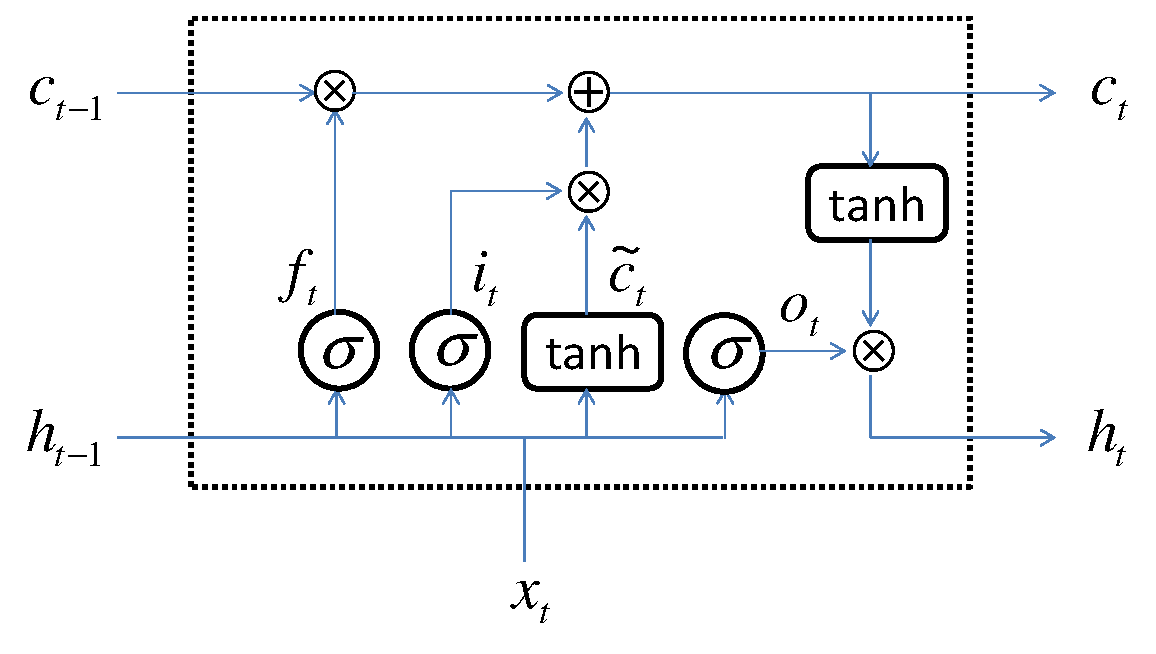
\includegraphics[width=80mm]{images/TsuruokaLab/lstm_yt.eps}
 \end{center}
 \caption{Long Short-Term Memory}
 \label{fig:lstm_yt}
\end{figure}

自然言語処理では,上述の問題点を解消し,高精度なリカレントニューラルネットワークを実現
する手法としてLSTM (Long Short-Term Memory) \cite{hochreiter1997long} や 
GRU (Gated Recurrent Unit) \cite{chung2014empirical} と呼ばれる
構造がよく用いられる.図\ref{fig:lstm_yt}に LSTM のユニットの構造を示す.
LSTM では,リカレントニューラルネットワークの通常の状態ベクトルで
ある $\boldsymbol{h}_{t}$ に加えて,メモリーセルと呼ばれる状態ベクトル $\boldsymbol{c}_{t}$ を持ち,
どのような情報をどのような場合に記憶(あるいは忘却)するかを細かく制御する「ゲート」と
呼ばれる機構を備えている.具体的には,LSTM の状態は,
\begin{eqnarray}
\boldsymbol{i}_t &=& \sigma(\boldsymbol{W}^{(i)} \boldsymbol{x}_t + \boldsymbol{U}^{(i)} \boldsymbol{h}_{t-1} + \boldsymbol{b}^{(i)})\\
\boldsymbol{f}_t &=& \sigma(\boldsymbol{W}^{(f)} \boldsymbol{x}_t + \boldsymbol{U}^{(f)} \boldsymbol{h}_{t-1} + \boldsymbol{b}^{(f)})\\
\boldsymbol{o}_t &=& \sigma(\boldsymbol{W}^{(o)} \boldsymbol{x}_t + \boldsymbol{U}^{(o)} \boldsymbol{h}_{t-1} + \boldsymbol{b}^{(o)})\\
\boldsymbol{\tilde{c}}_t &=& \sigma(\boldsymbol{W}^{(\tilde{c})} \boldsymbol{x}_t + \boldsymbol{U}^{(\tilde{c})} \boldsymbol{h}_{t-1} + \boldsymbol{b}^{(\tilde{c})})\\
\boldsymbol{c_t} &=& \boldsymbol{i}_t \odot \boldsymbol{\tilde{c}}_t + \boldsymbol{f}_t \odot \boldsymbol{c}_{t-1} \\
\boldsymbol{h_t} &=& \boldsymbol{o}_t \odot \tanh(\boldsymbol{c}_t)
\end{eqnarray}

\noindent
という式によって更新される.ただし,$\sigma(\cdot)$はシグモイド関数,$\odot$ はベクトルの要素積を表す.
$\boldsymbol{i}_t$,$\boldsymbol{f}_t$,$\boldsymbol{o}_t$ はそれぞれ,入力ゲート,忘却ゲート,出力ゲート
と呼ばれるベクトルであり,状態ベクトルの更新処理を制御する.

LSTM は,ニューラルネットワークを用いた自然言語処理で広く用いられており,いまでは多くの深層学習ライブラリで,
高性能なリカレントニューラルネットワークを実現する
標準的な「部品」として提供されている.本実験課題でも,LSTM を実験参加者が直接実装する必要はない.

%エンコーダーデコーダーモデルによる機械翻訳が成功したのはLSTMによるところが大きい.



\section{エンコーダ・デコーダモデル}

現在のニューラル機械翻訳技術のベースとなっているエンコーダ・デコーダモデル (encoder-decoder model) \cite{sutskever2014seq} 
では,2つのリカレントニューラルネットワークを使用する(図\ref{fig:encdec}).ひとつはエンコーダと呼ばれ,
翻訳元の文の単語を順次読み込み,文全体の内容を表す実数値ベクトルを生成する
役割を担う.もうひとつのリカレントニューラルネットワークはデコーダと呼ばれ,エンコーダ
が出力した実数値ベクトルを初期状態とし,上述の言語モデルと同様の仕組みで翻
訳先の単語列を出力する.
文全体の内容をひとつの実数値ベクトルで表現してしまおうというのはいかにも乱暴だが,
このような単純な仕組みで機械翻訳が実現できてしまうというのは驚きである.


\begin{figure}[t]
 \begin{center}
  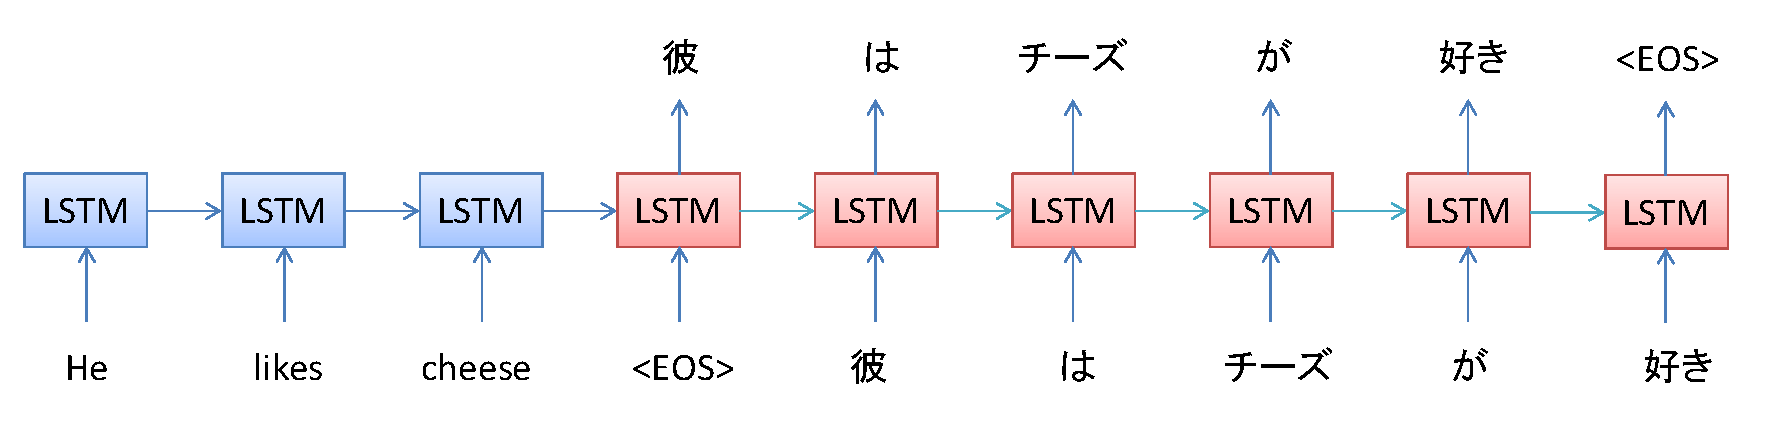
\includegraphics[width=140mm]{images/TsuruokaLab/encdec.eps}
 \end{center}
 \caption{エンコーダ・デコーダモデル}
 \label{fig:encdec}
\end{figure}

エンコーダ・デコーダモデルの学習は end-to-end で行う.つまり,エンコーダとデコーダを
それぞれ独立に学習されるのではなく,ひとつの大きなニューラルネットワークとして,
翻訳元の文から生成される翻訳先の単語列に関するモデルの対数尤度を最大化するようにパラメータ
を最適化する.


%\begin{equation}
%p(y_j | \boldsymbol{y}_{<j},\boldsymbol{x}) = \mbox{softmax}(\boldsymbol{W}_s s_j + b_s)
%\end{equation}

このような学習に必要なのは,「パラレルコーパス」と呼ばれる学習データである.
パラレルコーパスとは,文同士の
翻訳関係の対応がついている2言語のコーパスである.たとえば,機械翻訳モデル
の学習・評価用データとしてよく用いられるWMTデータセットでは,英仏では約3600
万文ペア,英独では約500万文ペアが提供されている.学習データの量が多ければ
多いほど翻訳精度が向上するというのは従来の統計的機械翻訳と同様だが,
ニューラル機械翻訳の場合は特にその傾向が強いと言われている.


\section{アテンション}

ニューラル機械翻訳のレベルを大きく引き上げたのは,アテンション(attention)と呼ばれ
る仕組みである \cite{bahdanau2015nmt}.これは,デコーダが各単語を出力する際の
情報として,エンコーダにおける各単語の隠れ状態の重み付き平均を入力として用いる
という方法で,翻訳元の文の文脈情報をより詳細にとらえることができるようになる.アテンションの
機構が導入されたことによってニューラル機械翻訳の精度は大きく向上し,従来の統計的機
械翻訳モデルの性能を凌駕することとなった.

\section{その他の応用}

Seq2seq モデルは,機械翻訳だけでなく様々な自然言語処理タスクに利用されている.
代表的な応用に,対話 \cite{vinyals2015neural},文書要約 \cite{rush2015neural},
質問応答 \cite{pmlr-v48-kumar16} などがある.

%\subsection{機械翻訳}



%\subsection{ニューラル会話モデル}



%\subsection{実験課題}


%https://github.com/chainer/chainer/tree/master/examples/seq2seq


\newpage
%!TEX root = ../main.tex
 \section{自然言語処理の実践}

 本節では,ニューラルネットワーク用フレームワークの Chainer を用いて自然言語を扱う方法を学ぶ.

 まず最初に,リカレントニューラルネットワークを用いた言語モデルの学習を行い,動作を確認する.その後,エンコーダー・デコーダモデルを用いた英日翻訳機を作成し,学習及び動作の確認を行う.

  \subsection{言語モデルの作成}
 まずはじめに,RNNを用いて日本語の言語モデルを学習する.「言語モデル」の詳しい説明は理論編を参照すること.

 なにはともあれまずはサンプルを実行してみよう.実験で使用するソースコードはサーバーのホームディレクトリに\verb+dl_exp_nlp.tar.gz+ という名前で配置されている.
  \begin{lstlisting}[basicstyle=\ttfamily\footnotesize, frame=single]
   $tar xzvf dl_exp_nlp.tar.gz
   $cd dl_exp_nlp
   $python language_model_rnn_train.py
  \end{lstlisting}
学習には10分前後かかるため,その間にプログラムの解説を行う.学習データは,datasetディレクトリ内の\verb+data_1000.txt+ を使用している.一行毎に,英文とそれに対応する日本語文がタブ文字で区切られて記入されている.また,それぞれの文は半角スペースで単語に区切られている.
\begin{itemize}
\item 学習データは,「田中コーパス」 (\url{http://www.edrdg.org/wiki/index.php/Tanaka_Corpus}) を加工したものである.
\item 「コーパス」とは,主に研究目的のため,自然言語のデータを体系的に収集し,構造化したデータのことを指す.
\item \verb+data_full.txt+ は田中コーパスの全てのデータであり,\verb+data_100.txt+ ,\verb+data_1000.txt+ はコーパスの中からそれぞれ100文,1000文を抜き出したものになっている.
\end{itemize}
学習データのパースを行っている\verb+sentence_data.py+ を見てみよう.自然言語処理の分野ではしばしば単語を「ID」で管理する.今回のプログラムでも,コーパス中の各単語にIDを割り振っている.日本語については\verb+SentenceData+ クラスの\verb+japanese_word_id()+ メソッドで「単語文字列$\rightarrow$単語ID」,\verb+japanese_word()+ メソッドで「単語ID$\rightarrow$単語文字列」の変換を行えるようになっている.また,\verb+japanese_sentence_data()+ メソッドはインデックスを与えると対応する文章データを返すが,これは「単語IDのリスト」という形式であることに注意する.なお,文の終端を表す EOS (End of Sentence) という概念が存在する.今回は EOS のIDを0と定義した.

  \begin{figure}[htb]
   \centering
   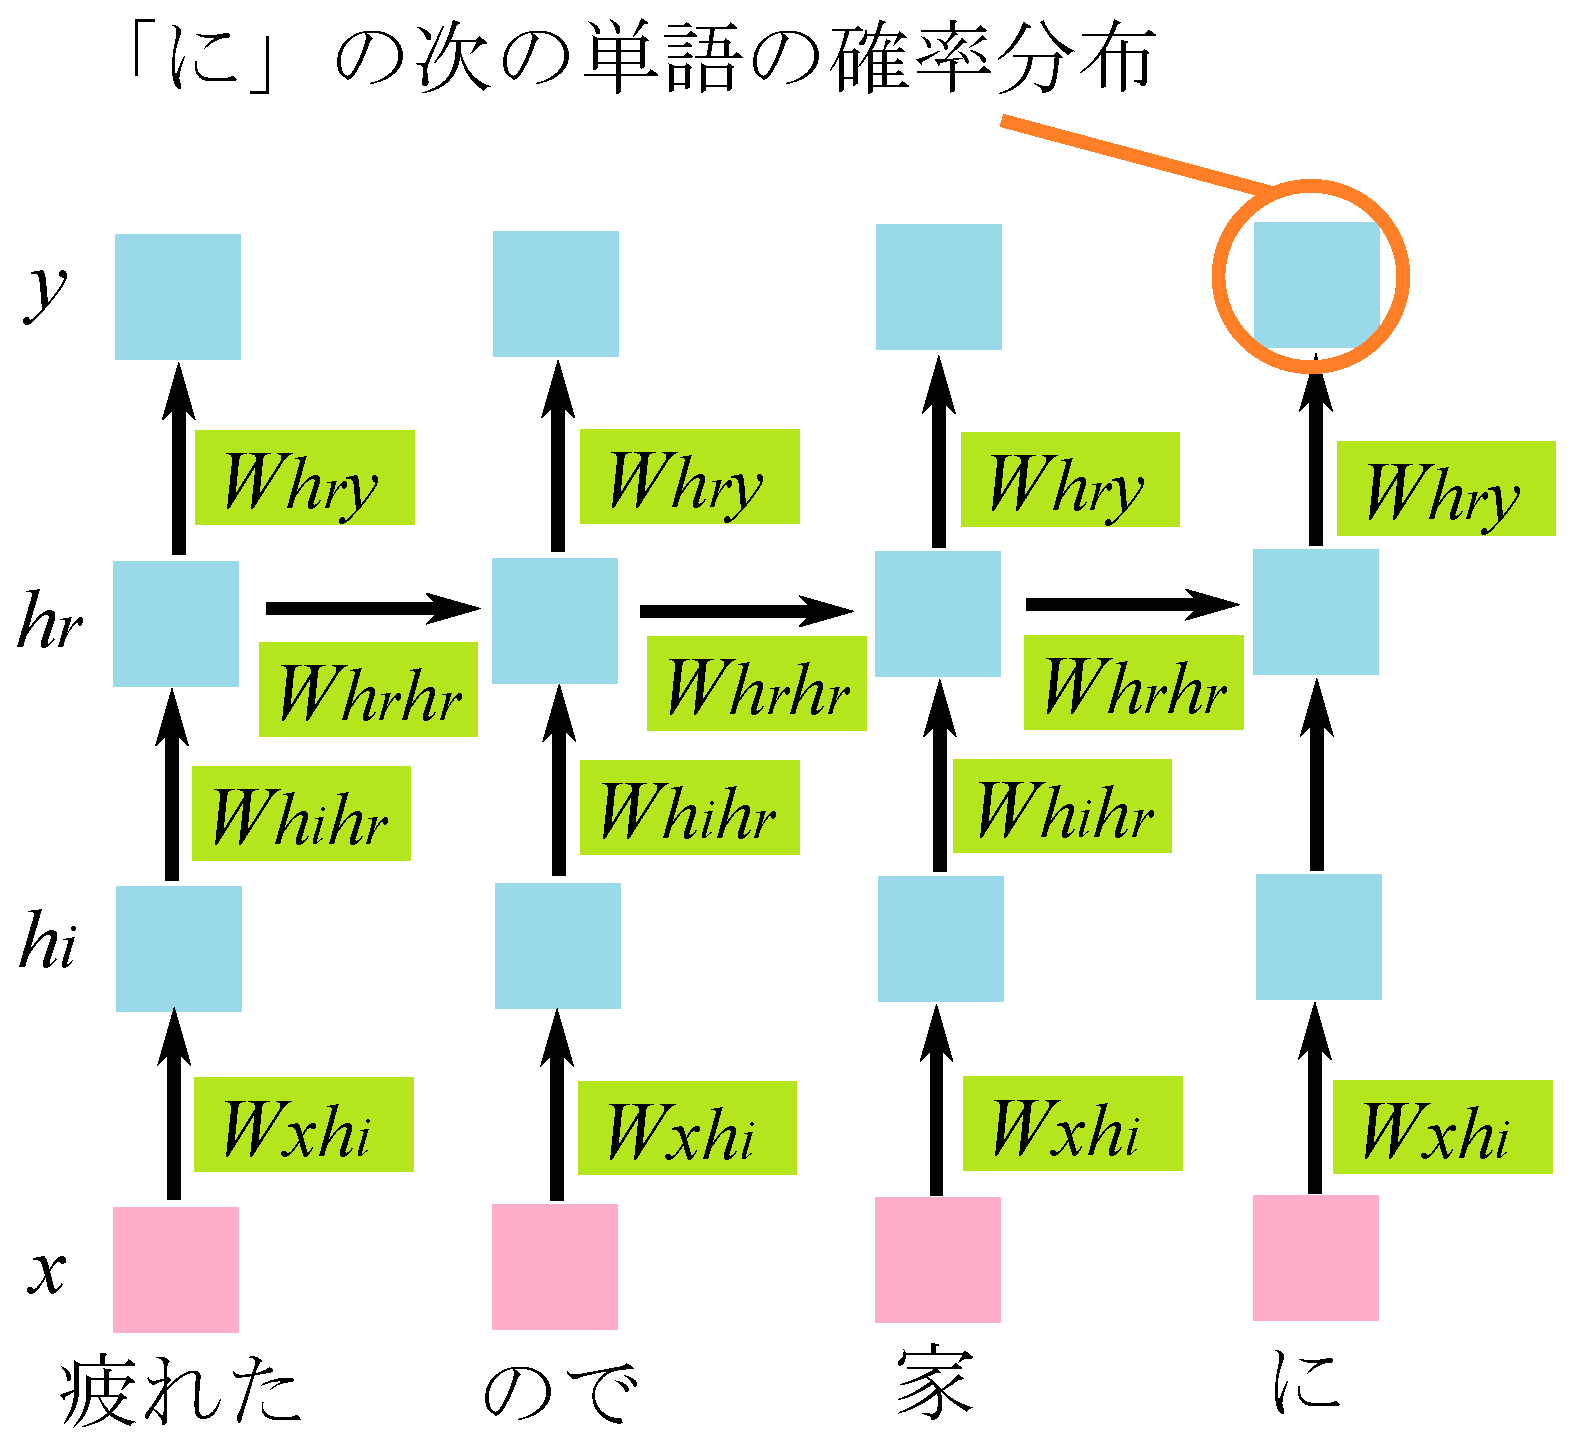
\includegraphics[width=80mm]{images/TsuruokaLab/langmodel.eps}
   \caption{RNN を用いた言語モデル}
   \label{fig:langmodel}
  \end{figure}

次に\verb+language_model_rnn.py+ を読む.\verb+LanguageModel+ というクラスが定義されており,\verb+chainer.Chain+ クラスを継承している.\verb+chainer.Chain+ はニューラルネットワークのモデルを表現するためのクラスであり,ネットワークのパラメータを\verb+chainer.Chain+ の\verb+__init__+ に渡している.今回用いるのは図\ref{fig:langmodel}に示すネットワークである.$x$は単語IDを表現するベクトルで,語彙数に等しい次元を持ち,単語IDに対応する位置の要素のみ1で,他の要素は0になっている.このようなベクトルを one hot vector と呼ぶ.本来ならばニューラルネットワークの入力としてはこの one hot vector を用いなければならないが,Chainer には one hot vector を扱うための\verb+EmbedID+ というクラスが存在する.このクラスは,入力に one hot vector の代わりに単一の整数を取ることができ,指定した整数の位置が1となる one hot vector として扱ってくれる.今回は$W_{xh_i}$が\verb+EmbedID+ になる.$W_{xh_i}$は,単語IDに対応する$h_i$の組が横に並んだ行列と見ることもできる.\verb+Linear+ クラスは単なる行列である.\verb+EmbedID+ や\verb+Linear+ には初期化時に入力の次元と出力の次元を渡す必要がある.

また,今回はリカレントニューラルネットワークとして,隠れ層$h_r$の値を保存する必要があるため,メンバとして$h_r$の値を持っており,\verb+reset_state()+ メソッドで初期化できるようにしている.\verb+__call__+ により,単語IDを入力として受け取りネットワークの出力を返す.出力は,語彙数の次元を持ち,各単語IDに対応する位置の値が,その単語の出現確率を示している.
\begin{itembox}[l]{softmax}
より正確には,出力ベクトルに softmax と呼ばれる処理を行うことで,ベクトルの要素を確率に変換する.
\end{itembox}


\verb+language_model_rnn_train.py+ で実際に学習を行っている.学習データ全体を一周すると「1 epoch」となり,今回はデフォルトでは 10 epochs の学習を行う.学習結果は 1 epoch 毎に,\verb+trained_model+ ディレクトリ以下に保存される.

さて,そろそろ学習が終わっただろうか.学習が終了したら,\verb+language_model_rnn_test.py+ を実行することで,学習した言語モデルをテストすることができる.
  \begin{lstlisting}[basicstyle=\ttfamily\footnotesize, frame=single]
   $python language_model_rnn_test.py
  \end{lstlisting}
として実行し,最初の単語,例えば「私」と入力すると,2単語目に来る確率が最も高い単語が出力される.さらに,「入力した1単語目,推定された2単語目」という単語列から,最も確率の高い3単語目が続けて出力され,文の終端である EOS が出力されるまで,再帰的に推定を行う.入力には半角スペースで区切った複数単語を入れることもでき,「私 は ここ」と入力した場合は,最も確率の高い4単語目から推定が行われる.
 \begin{practice}
   適当な単語または単語列を入力し,入力によって出力が変化すること,ある程度「日本語らしい」文章になることを確認せよ.
 \end{practice}
 \newpage

  \subsection{Long Short-Term Memory (LSTM)}
 理論編で学んだように,単純な RNN で精度の良い学習を行うのは難しく,LSTM や GRU 等の改良された構造が用いられることが多い.ここでは LSTM を使用して先程と同様に言語モデルの学習を行う.

  \begin{figure}[htb]
   \centering
   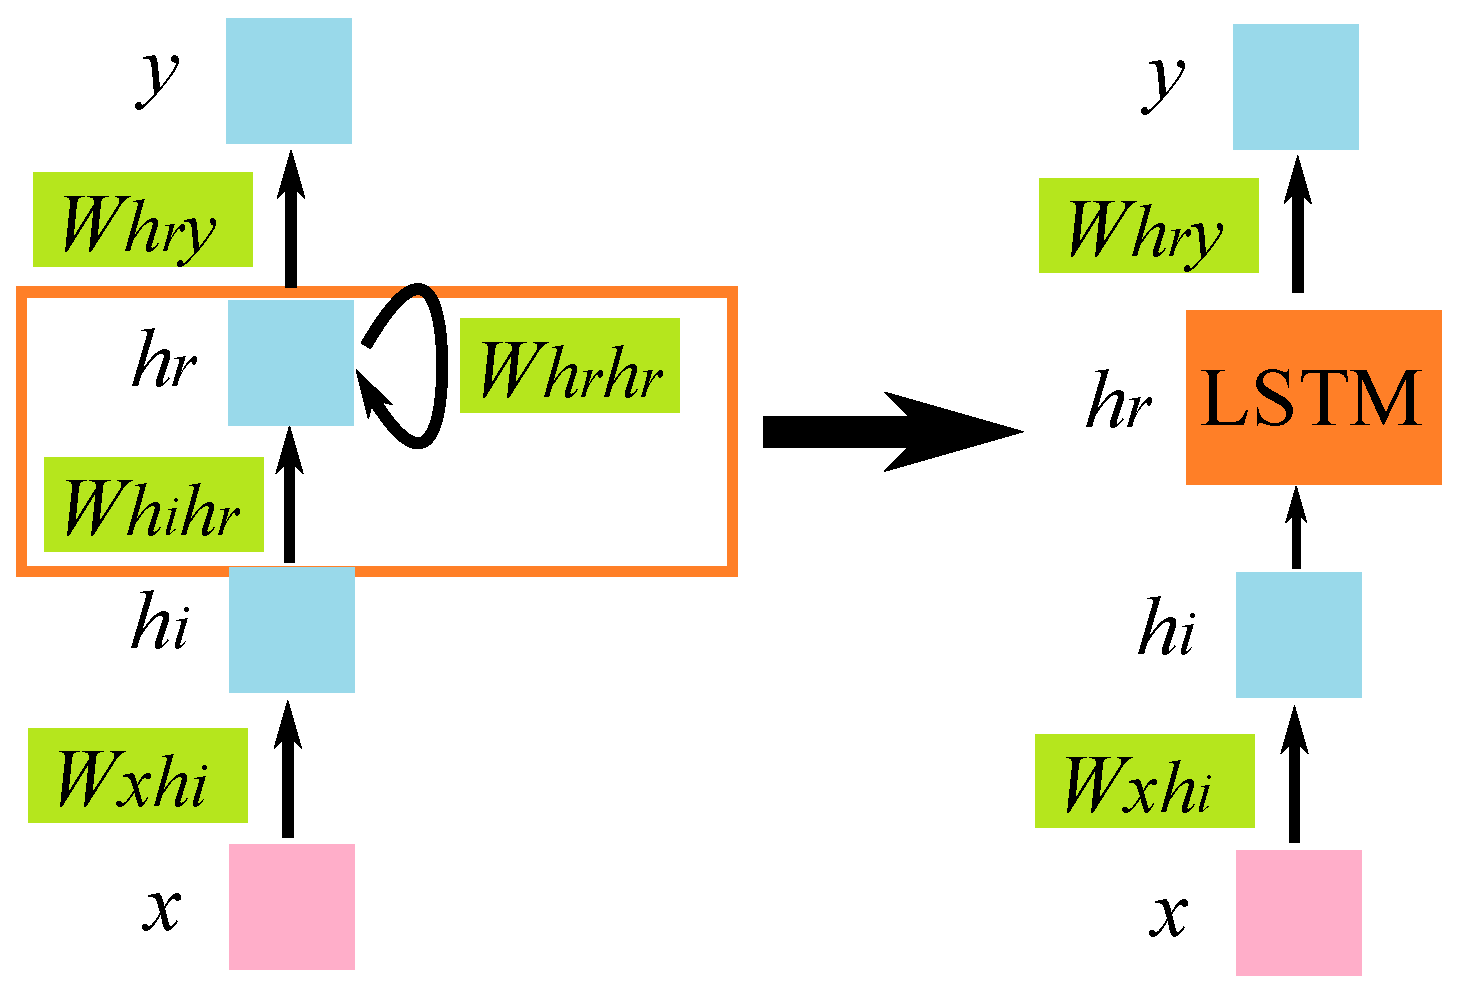
\includegraphics[width=80mm]{images/TsuruokaLab/lstm.eps}
   \caption{ChainerのLSTMクラスによる RNN の置き換え}
   \label{fig:lstm}
  \end{figure}

 Chainer には既に LSTM のモデルが用意されている.図\ref{fig:lstm}に示すように,RNN 部分をまるごと置き換えるようになっており,隠れ層のデータも含まれている.\verb+language_model_lstm.py+ に,LSTM を用いて言語モデルの学習を行う例を示した.RNN を自分で実装したときとは異なり,\verb+reset_state()+ メソッドでは,\verb+chainer.links.LSTM+ の\verb+reset_state()+ メソッドを呼び出す様になっている.これは,隠れ層のデータは\verb+chainer.links.LSTM+ の内部に含まれているからである.さて,今回は\verb+LanguageModel+ クラスの\verb+__call__+ の実装をまだ行っていない.\verb+language_model_rnn.py+ も参考にしつつ,各自で実装してみよ.
 \begin{practice}
 \verb+language_model_lstm.py+ における\verb+LanguageModel+ クラスの\verb+__call__+ を実装し,実際に学習を行ってみよ.学習は\verb+language_model_lstm_train.py+ を実行することで行うことができる.学習が終了したら,\verb+language_model_lstm_test.py+ を実行し,動作を確認せよ.
 \end{practice}
 \begin{practice}
  \verb+language_model_lstm_train.py+ 及び\verb+language_model_lstm_test.py+ を書き換え,英語の言語モデルを学習し,動作を確認せよ.学習には時間がかかるため,学習中に次の章を読み進めておくと良い.
 \end{practice}

  \subsection{エンコーダー・デコーダモデル}
 次に,エンコーダー・デコーダモデルを用いた英日翻訳機の学習を行う.エンコーダー・デコーダモデルについては理論編を参照すること.LSTM を用いた英日翻訳の例を図\ref{fig:encdecexample}に示す.\verb+translator_model.py+ を読むと,このモデルが定義されている.注意点として,Chainer の\verb+LSTM+ クラスは隠れ層のデータを内部に保持している.今回は隠れ層のデータをエンコーダ用LSTMからデコーダ用LSTMに引き継ぐ必要があるため,\verb+LSTM+ クラスの代わりに\verb+StatelessLSTM+ クラスを用いた.\verb+StatelessLSTM+ は,隠れ層のデータを内部に持たず,外部に変数として保存して計算時に与えるようになっている.また理論編で学んだように,LSTMは隠れ層の他にメモリーセルと呼ばれる状態ベクトルも持つため,これも隠れ層と同様に変数として保存する必要がある.

  \begin{figure}[htb]
   \centering
   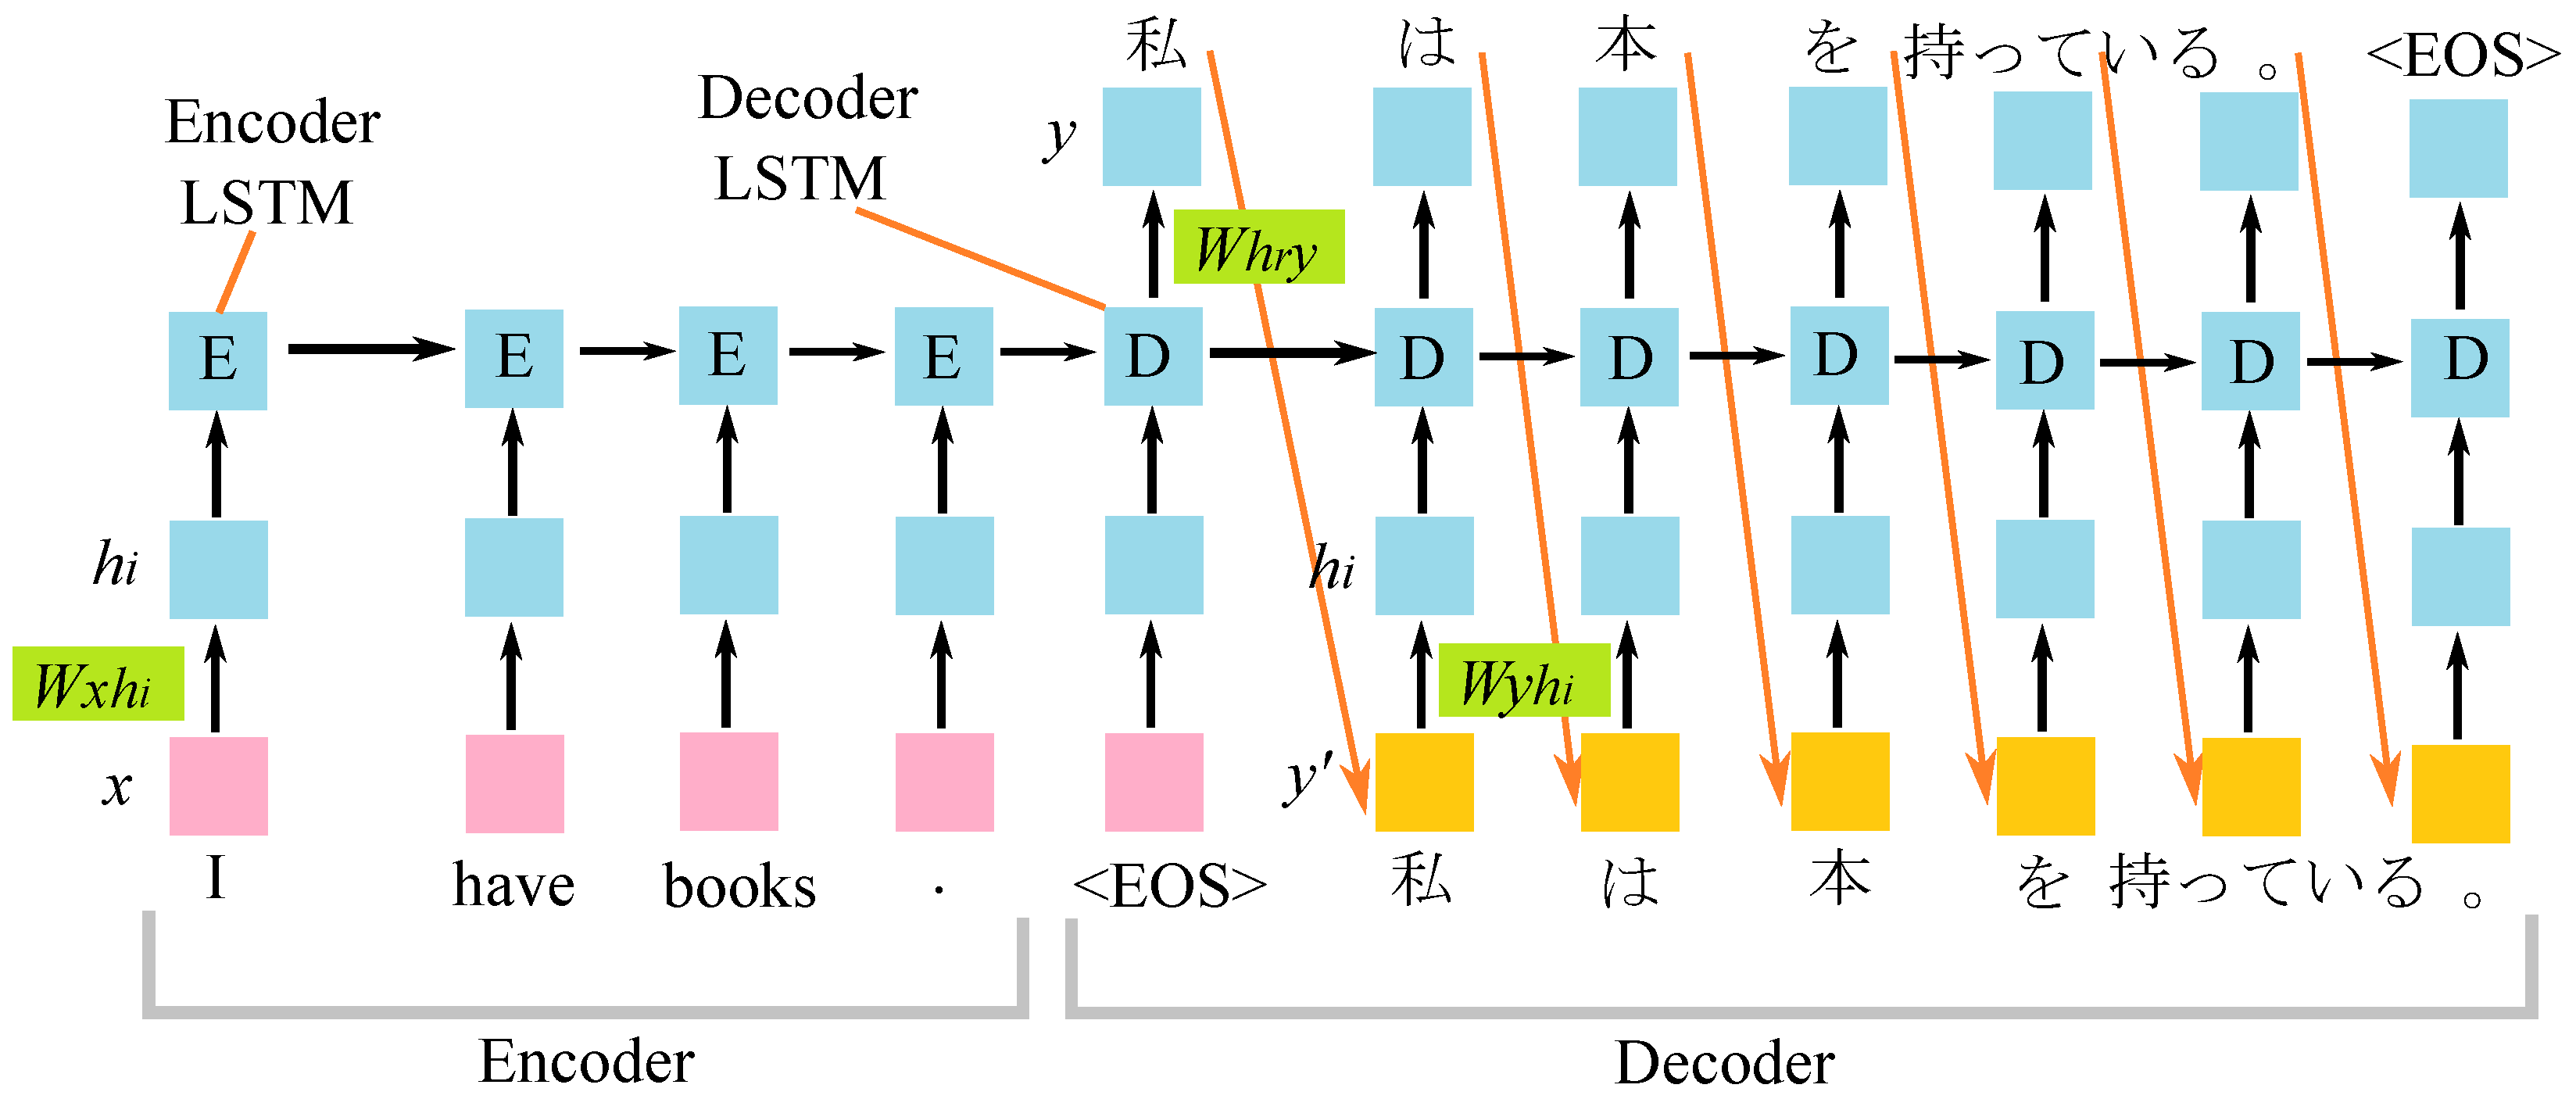
\includegraphics[width=130mm]{images/TsuruokaLab/encdecexample.eps}
   \caption{エンコーダー・デコーダモデルによる英日翻訳}
   \label{fig:encdecexample}
  \end{figure}

 \begin{practice}
  \verb+translator_model_train.py+ を実行し,翻訳モデルの学習を行ってみよ.学習している間に,\verb+translator_model.py+ 及び\verb+translator_model_train.py+ を読んで,ネットワークを定義している部分,エンコードやデコードを行う部分などを探してみよ.
 \end{practice}
 \begin{practice}
  学習が終了したら,\verb+translator_model_test.py+ を実行し,結果を確かめてみよ.入力の際は「I have a book .」のように,ピリオドも単語として区切るため,スペースを挟む必要があることに注意する.
 \end{practice}

大抵の場合,一見日本語のような文章ではあるが,翻訳結果としては間違った文章が出力されたと思われる.これは主に学習データの数が足りないためである.今回は1000文の学習データを用いて 10 epochs の学習を行ったが,この数では正確な翻訳は不可能である.\verb+traind_model/translator_full.model+ は,\verb+data_full.txt+ を用いて約15万文で 10 epochs の学習を行ったデータである.\verb+translator_model_test_full.py+ を実行することで,このデータを用いて翻訳を行うことができる.
 \begin{practice}
  \verb+translator_model_test_full.py+ を実行し,動作を確認せよ.
 \end{practice}

  \subsection{未知語対応}
 今までのプログラムで作成したモデルでは,コーパスに含まれない単語が入力された場合に対応できなかった.そこで,未知の単語が入力された場合でもある程度動作する仕組みを考える.簡単な例としては,未知の単語を共通の「\textless UNKNOWN\textgreater 」という単語に置き換えてしまうという手法が考えられる.この手法を動作させるには,学習の際に「\textless UNKNOWN\textgreater 」を含むデータセットが必要になる.そのため,データセットを読み込む際に変換を行う.変換方法の例としては
\begin{itemize}
\item 出現回数が一定回数以下の単語を全て「\textless UNKNOWN\textgreater 」に置き換える.
\item 各単語が初めて出現したときに「\textless UNKNOWN\textgreater 」に置き換える.
\end{itemize}
等が考えられる.「\textless UNKNOWN\textgreater 」を扱うための準備として,\verb+sentence_data.py+ に
  \begin{lstlisting}[basicstyle=\ttfamily\footnotesize, frame=single]
UNKNOWN_WORD_ID = 1
  \end{lstlisting}
を追記し,また単語の辞書作成部分は
  \begin{lstlisting}[basicstyle=\ttfamily\footnotesize, frame=single]
    self.en_word_to_id = {"<EOS>":EOS_ID, "<UNKNOWN>":UNKNOWN_WORD_ID}
    self.en_word_list = ["<EOS>", "<UNKNOWN>"]
    self.jp_word_to_id = {"<EOS>":EOS_ID, "<UNKNOWN>":UNKNOWN_WORD_ID}
    self.jp_word_list = ["<EOS>", "<UNKNOWN>"]
  \end{lstlisting}
とする.
 \begin{practice}
  \verb+sentence_data.py+ の\verb+__init__+ で学習データを読み込んでいる部分を書き換え,データセットに「\textless UNKNOWN\textgreater 」が含まれるようにせよ.
 \end{practice}
 \begin{practice}
  \verb+language_model_lstm_test.py+ や,\verb+translator_model_test.py+ を書き換え,未知の単語が入力された場合に「\textless UNKNOWN\textgreater 」に置き換えて,出力が得られるようにせよ.これをテストする場合は,前の課題で書き換えた\verb+sentence_data.py+ を用いて学習をやり直す必要があることに注意せよ.
 \end{practice}

  \subsection{発展課題}
余力のある人は,以下の発展課題に取り組んでみよ.
\begin{itemize}
\item いくつかの学習データをまとめて学習することで,主にGPUを使用する場合の学習効率を上げることができる.この手法を mini batch と呼ぶ.Chainer では入力データの次元を挙げることで簡単に mini batch 化が可能であるが,系列データはデータによってデータ長が異なるため,少々面倒である.Chainer には可変長データをバッチ化しやすくするために NStepLSTM というクラスがある.NStepLSTM の使い方を調べ,実験で用いたプログラムを mini batch 化せよ.
\item 今回は単語IDから特長ベクトル$h_i$を生成するための行列$W_{xh_i}$も同時に学習したが,各単語を表す特徴ベクトルを事前に学習することも可能である.学習済みのデータを公開している人も多いので,それらのデータを用いるように今回のプログラムを変更してみよ.Word embedding や, Word2Vec 等のキーワードで検索すると良い.
\item 配布したデータセットは,前述のように田中コーパス (\url{http://www.edrdg.org/wiki/index.php/Tanaka_Corpus}) を加工したものであるが,加工前のコーパスデータには,単語の原型などの追加データが存在する.それらのデータを上手く使うことで,学習の効率や精度を上げることができないか検討せよ.なお,今回英単語の切り分けには Stanford CoreNLP (\url{https://stanfordnlp.github.io/CoreNLP/}) を用いた.
\item ネットワークの構造を変更することで,より精度良く学習が行なえないか検討せよ.例えば,理論編で学んだ attention を導入してみよ.
\end{itemize}

  \subsection{自由課題のヒント}
\begin{itemize}
\item エンコーダー・デコーダモデルの用途は翻訳に限らず,系列データの入力から系列データを出力する一般のタスクに応用できる.例えば,長い文章を入力すると要点をまとめて短くしてくれるような要約タスクなどが考えられる.
\item RNN の入力や出力は単語(列)に限らない.例えば画像分野と組み合わせて,連続画像を入力としたり,画像から文章を生成する等の応用も考えられる.
\end{itemize}
 

% 強化学習部分
\chapter{Reinforcement Learning}



%\section{強化学習}

本実験課題では,近年の人工知能研究において様々な場面で用いられている,
強化学習 (reinforcement learning) についてその基本的な原理と動作を学ぶ.

強化学習が有用な例として,与えられた環境の中で「賢く」行動するロボットのAI (以下,エージェントと呼ぶ)
を作ることを考えてみよう.そのようなエージェントを実現するもっとも素朴な方法として,
「X という状態のときには Y する」といったようなルールをひたすら書き連ねたプログラムを書く,という
アプローチが考えられる.しかし,このような「ルールベース」の方法は,
少し環境が複雑になるとすぐに破綻する.そこで,強化学習では,人間が明示的に
エージェントの行動のためのルールを教えるのではなく,
エージェント自身に多数の試行錯誤をさせ,その経験を通して適切な行動基準を見つけさせる
というアプローチをとる.
人間は,エージェントが適切な行動をした場合には,プラスの「報酬」を与え,不適切な
行動をした場合にはマイナスの報酬を与える.報酬は必ずしも各行動ごとに与える必要はなく,
どのように行動すれば(長い目で見て)報酬を最大化できるのかについてはエージェント自身が考える,
というのが強化学習の特徴である.

近年,強化学習は様々な分野で応用が進んでいる.ブロック崩しやインベーダーゲームといった簡単な
ビデオゲームをプレイすることのできるAI \cite{mnih2015humanlevel} や,人間の棋譜を一切使わずにきわめて高い棋力
を達成した囲碁プログラム \cite{silver2017go} などのニュースは記憶に新しい.

\section{マルコフ決定過程}

\begin{figure}[t]
 \begin{center}
  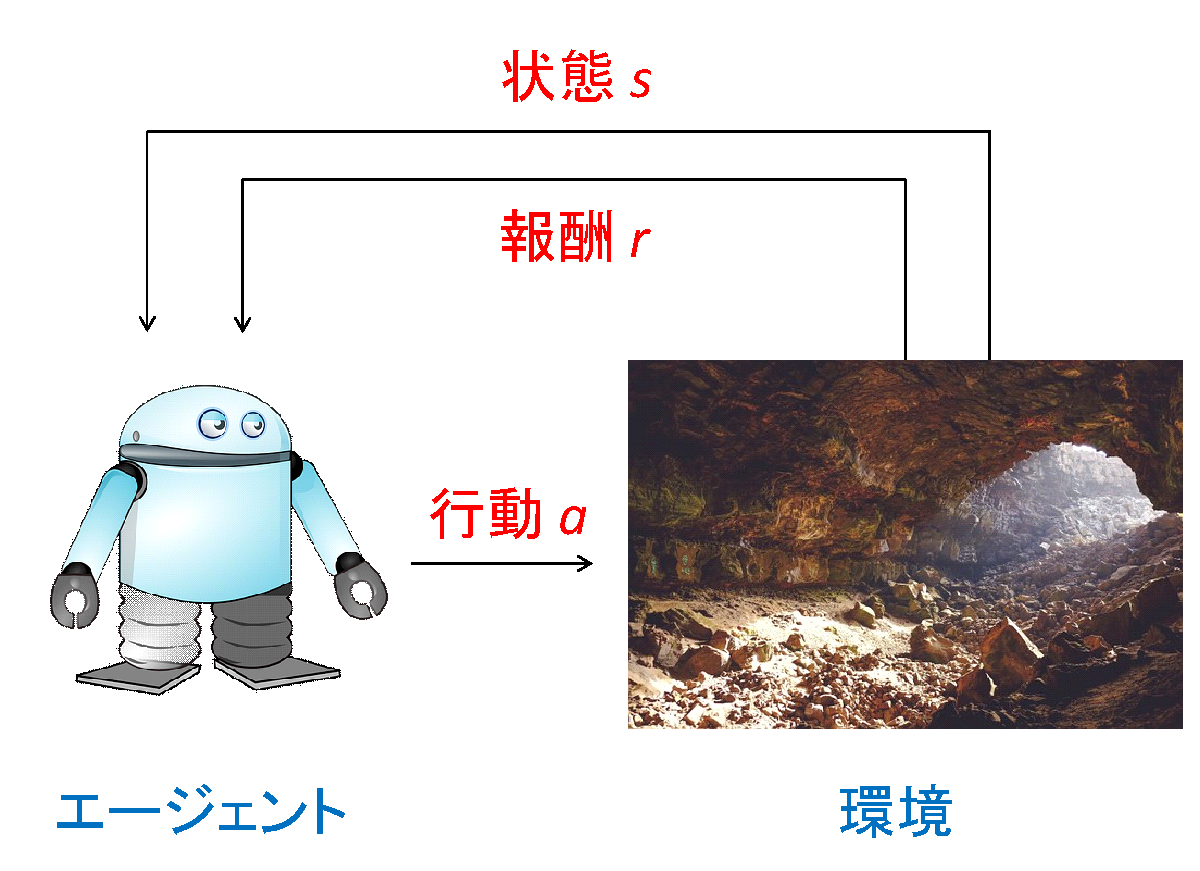
\includegraphics[width=80mm]{images/TsuruokaLab/rl.eps}
 \end{center}
 \caption{強化学習}
 \label{fig:rl1}
\end{figure}

強化学習を考える上での基本的な枠組みであるマルコフ決定過程 (Markov decision process, MDP) 
について簡単に述べる.マルコフ決定過程とは,
\begin{itemize}
\item 状態 (state) の有限集合 $S$
\item 行動 (action) の有限集合 $A$
\item 状態遷移関数 $P(s'|s,a)$: 状態$s \in S$ において行動$a \in A$をとった場合に状態$s' \in S$ に遷移する確率
\item 報酬関数 $R(s,a,s')$: 状態$s$から行動 $a$ によって状態$s'$ に遷移したときに得られる報酬
\end{itemize}
\noindent
によって構成され,エージェントの環境 (environment) を規定する.

いま,図\ref{fig:rl1} に示すように,この環境の中で,時刻 $t$ において状態 $s_t$ にあるエージェントが,行動 $a_t$ を選択したとする.
その結果,状態は $s_{t+1}$ に変化し,同時にエージェントは報酬 $r_{t+1}$ を受け取る.
強化学習におけるエージェントの目的は,現在から未来にわたる累積報酬

\begin{equation}
g_t = r_{t+1} + \gamma r_{t+2} + \gamma^2 r_{t+3} + \ldots = \sum_{k=0}^{\infty} \gamma^k r_{t+k+1}
\end{equation}

\noindent
を最大化する行動を選択することだと定式化される.$\gamma$ は割引率 (discount factor) 
と呼ばれる値であり,現時点ですぐに
もらえる報酬を未来の報酬よりもどれだけ重視するかを決めるパラメータである.

\section{Q学習}

強化学習のためのアルゴリズムとして最もよく知られているもののひとつに,Q学習 (Q-learning) と呼ばれる
アルゴリズムがある.いま,状態 $s$ のときに行動 $a$ を取り,その後,最善の行動を取り続けた場合に
得られる累積報酬の期待値を $Q^*(s,a)$ と書くものとする.$Q^*(s,a)$ は,Bellman 方程式と呼ばれる
以下の再帰的な関係式を満たす.
\begin{equation}
Q^*(s,a) = \sum_{s'} P(s'| s, a) (R(s, a, s') + \gamma \max_{a'} Q^*(s', a') )
\end{equation}

もし,任意の $s$ と $a$ の組み合わせに対して  $Q^*(s,a)$ がわかっているのであれば,
状態$s_t$において,エージェントは, $Q^*(s_t, a_t)$ が最大の行動 $a_t$ を選択すれば
累積報酬を最大化することができる.つまり,エージェントの行動選択の問題が解けたことになる.

もちろん通常は $Q^*(s,a)$ は未知なので,何らかの方法で推定する必要がある.
Q学習では,エージェントが環境のなかで行動するたびに,以下の更新式にしたがって
 $Q^*(s,a)$ の推定値である $Q(s,a)$ を更新する.
\begin{equation}
Q(s_t, a_t) \leftarrow Q(s_t, a_t) + \alpha [ r_{t+1} + \gamma \max_a Q(s_{t+1},a) - Q(s_t, a_t) ]
\end{equation}

%この更新式は次のように書かれることもある.
%
%\begin{equation}
%Q(s_t, a_t) \leftarrow (1 - \alpha) Q(s_t, a_t) + \alpha [ r_{t+1} + \gamma \max_a Q(s_{t+1},a) ]
%\end{equation}
%
%いずれにせよ,$Q(s_t, a_t)$ を

すなわち,$Q(s_t, a_t)$ を
\begin{equation}
r_{t+1} + \gamma \max_a Q(s_{t+1},a)
\end{equation}

\noindent
に近づけるように更新する.ただし,$\alpha \in [0,1]$ は学習率と呼ばれるパラメータである.Q学習では,
エージェントが全ての状態をゼロ以上の確率で訪れるように行動する場合,
学習率を徐々に下げていくことにより,$Q(s,a)$ が $Q^*(s,a)$ に収束することが知られている.


\begin{figure}[t]
 \begin{center}
  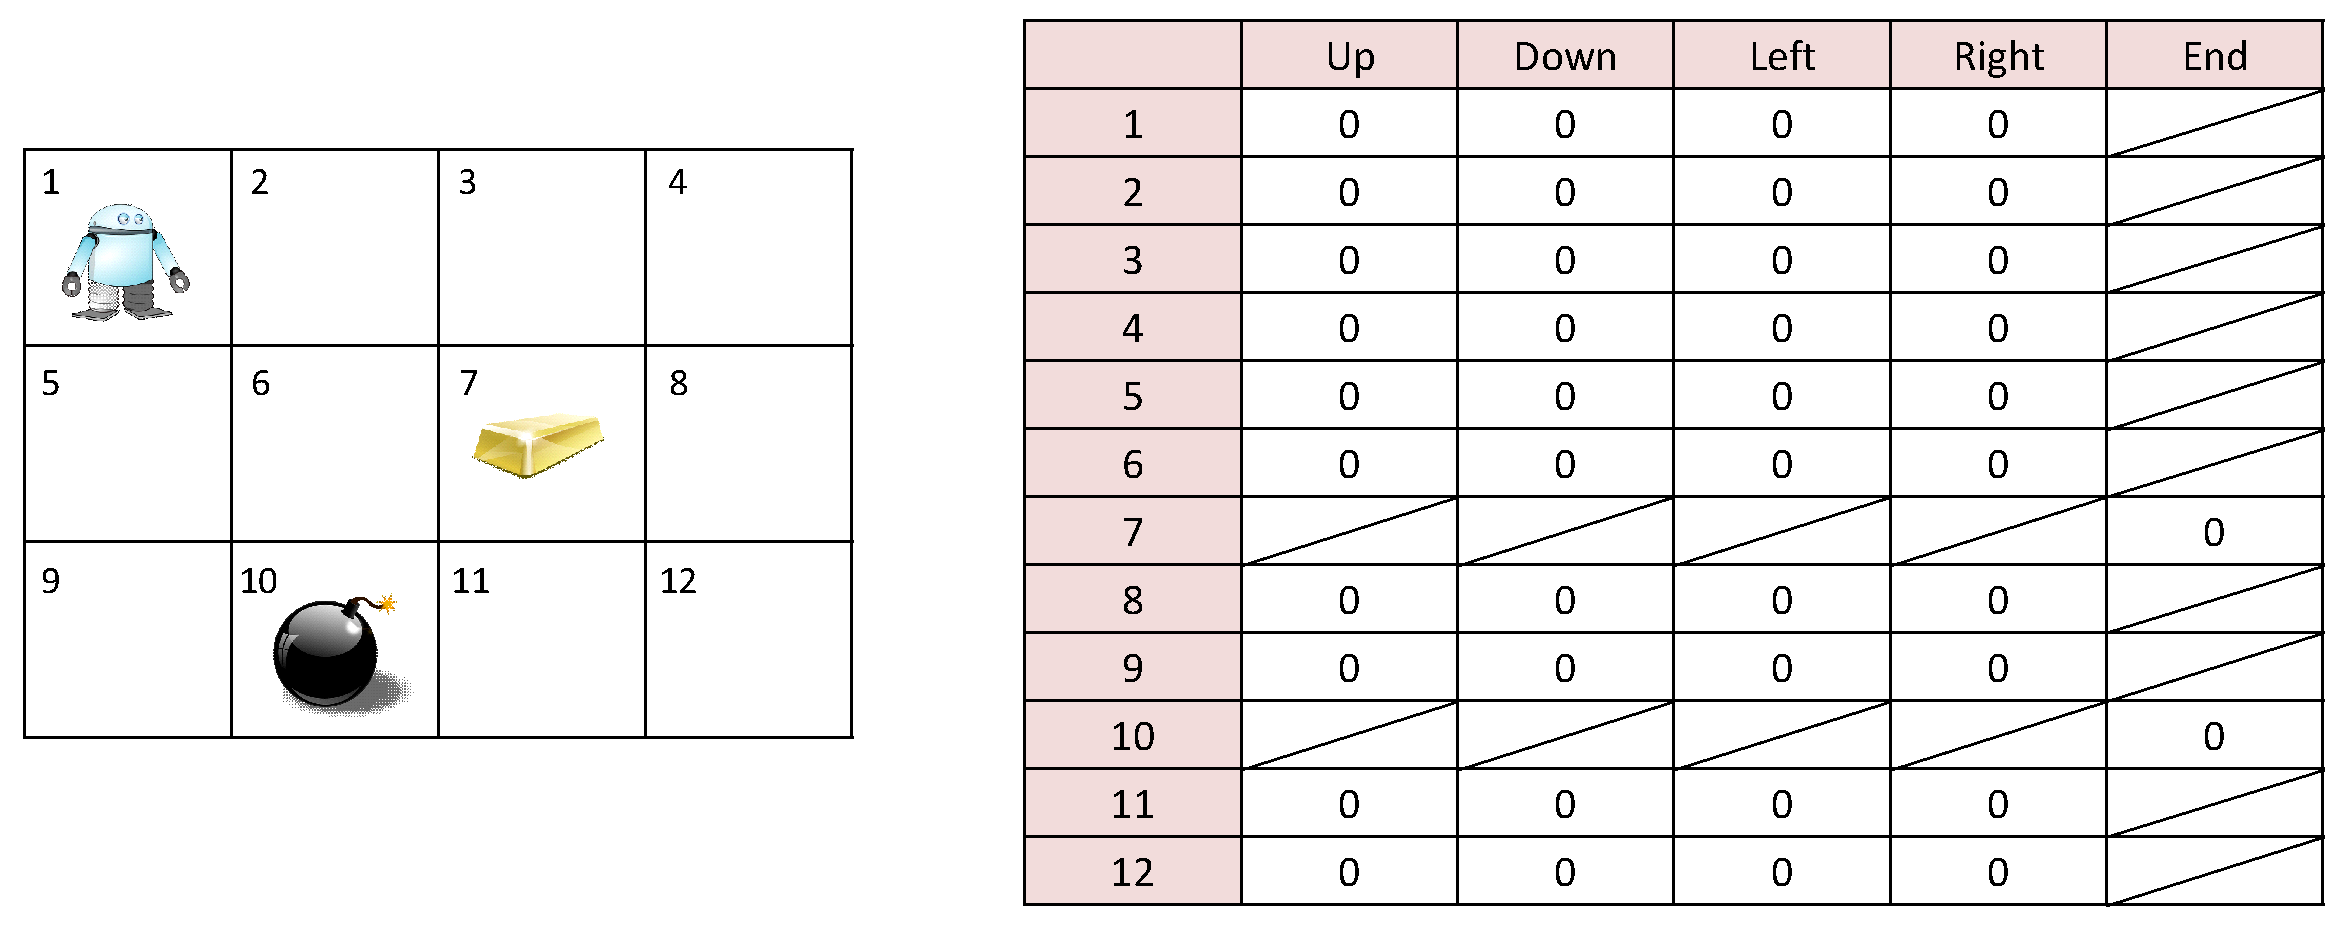
\includegraphics[width=140mm]{images/TsuruokaLab/ql1.eps}
 \end{center}
 \caption{Q学習(初期状態)}
 \label{fig:ql1}
\end{figure}

\subsection{テーブルを用いたQ学習の例}

Q学習の様子を例を用いて説明しよう.この例では,学習率$\alpha$は常に$1.0$,割引率$\gamma$ は $0.9$ 
であるとする.

図\ref{fig:ql1}に学習の初期状態を示す.エージェントは状態1から出発するものとする.
また,エージェントは各状態において Up, Down, Left, Right の4つの行動をとることができる.
ただし,状態7と状態10では,End という行動しかとることができず,それぞれ
$100$もしくは$-100$の報酬を受け取ったのち,エピソードが終了する.図の右側に示すテーブルは,
$Q(s,a)$ を表し,すべてゼロで初期化されている.

この状態からエージェントがランダムに行動した結果,状態7に到達したとする.すると,次のステップでは
行動として End をとり,報酬100を受け取り,エピソードが終了するため,更新式
\begin{equation}
Q(7, \mbox{End}) \leftarrow Q(7, \mbox{End}) + 1.0 \times [ 100 + 0.9 \times 0 - 0 ]
\end{equation}

\noindent
によって,$Q(7, \mbox{End})$ の値が 100 に更新される.次のエピソードで,状態10に到達した場合,
報酬として $-100$ を受け取るため,同様の計算により $Q(10, \mbox{End})$ の値は $-100$ となる.
この時点での$Q(s,a)$の値を格納するテーブルの状態を図\ref{fig:ql2}に示す.


\begin{figure}[t]
 \begin{center}
  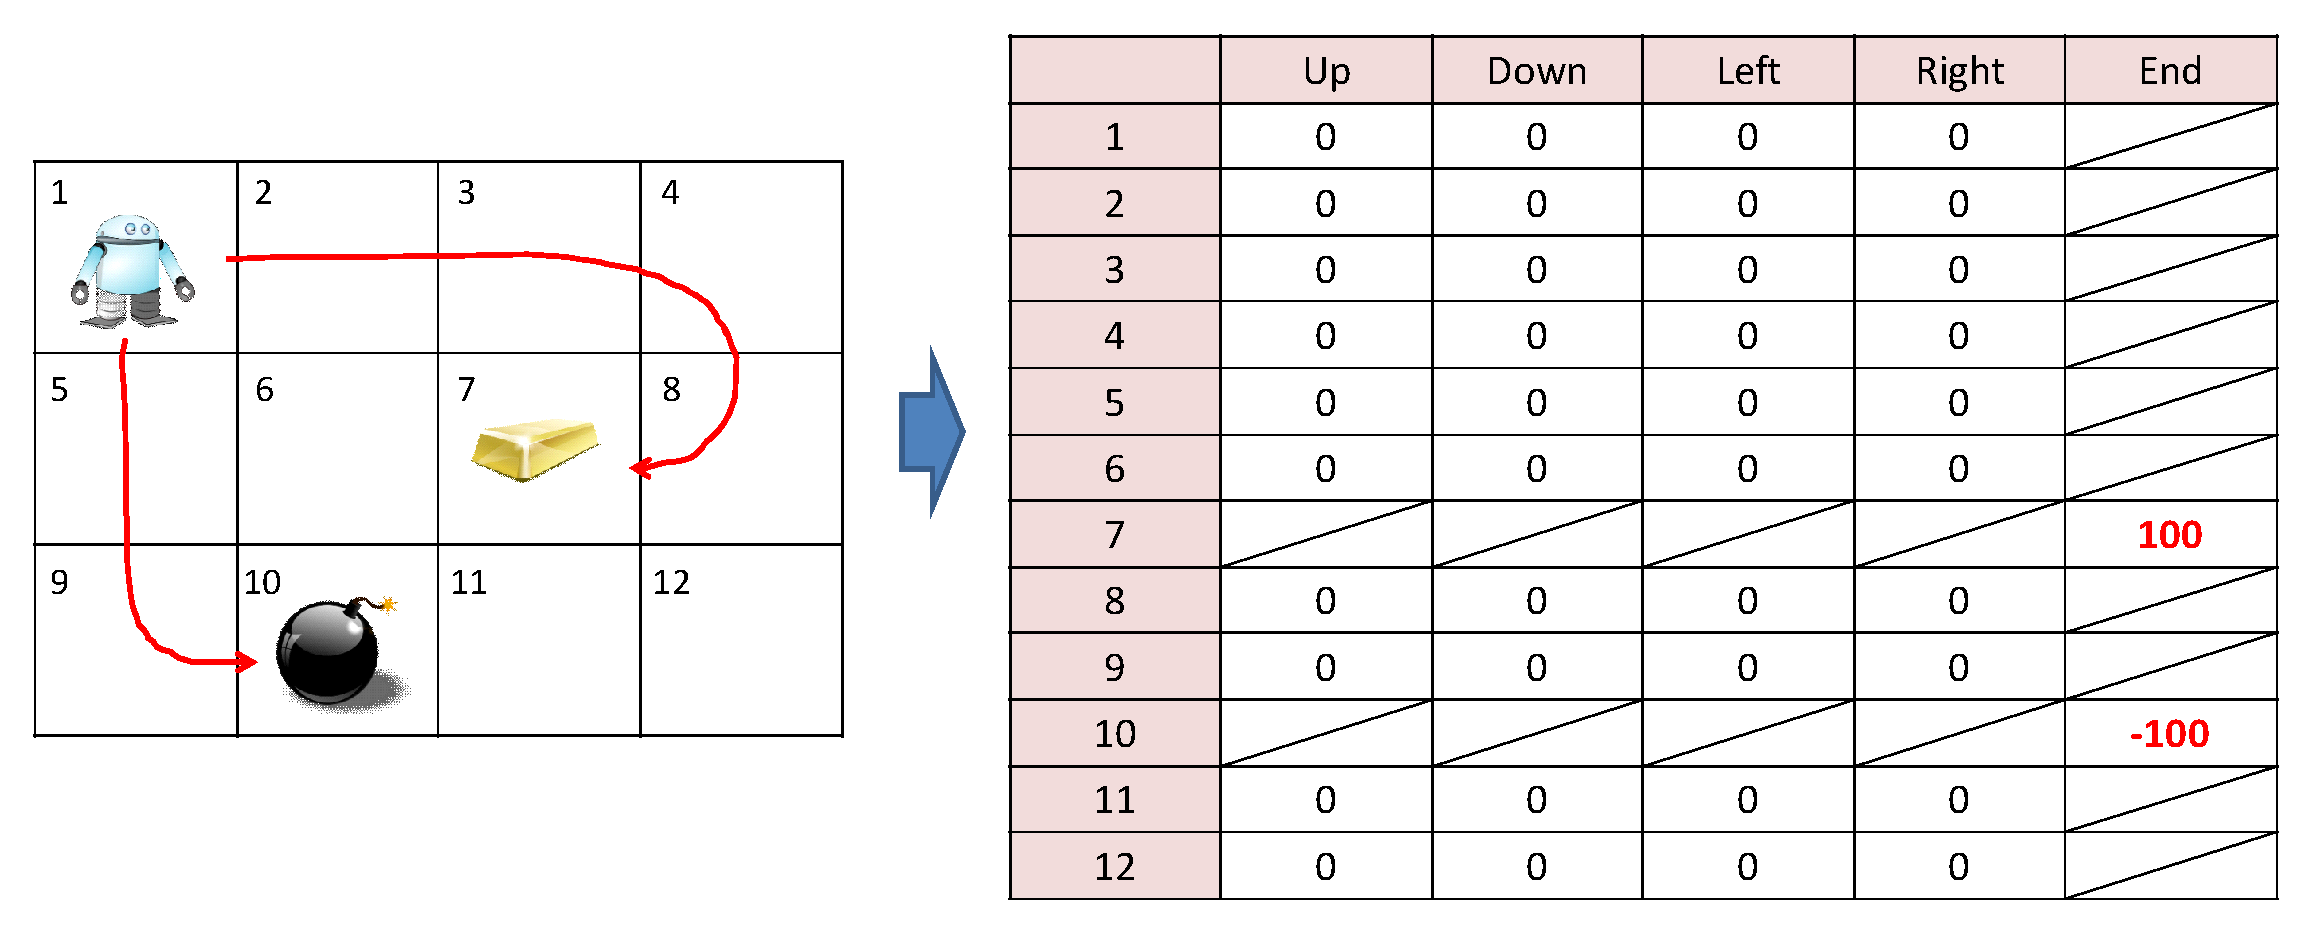
\includegraphics[width=140mm]{images/TsuruokaLab/ql2.eps}
 \end{center}
 \caption{Q学習(状態7と状態10を経験した後)}
 \label{fig:ql2}
\end{figure}

その後,エージェントは図\ref{fig:ql3} に示すように,状態3を経由して状態7に到達したとする.
この場合,更新式は,
\begin{equation}
Q(3, \mbox{Down}) \leftarrow Q(3, \mbox{Down}) + 1.0 \times [ 0 + 0.9 \times 100 - 0 ]
\end{equation}
\noindent
となるため,$Q(3, \mbox{Down}) $ の値が 90 に更新されることになる.


\begin{figure}[t]
 \begin{center}
  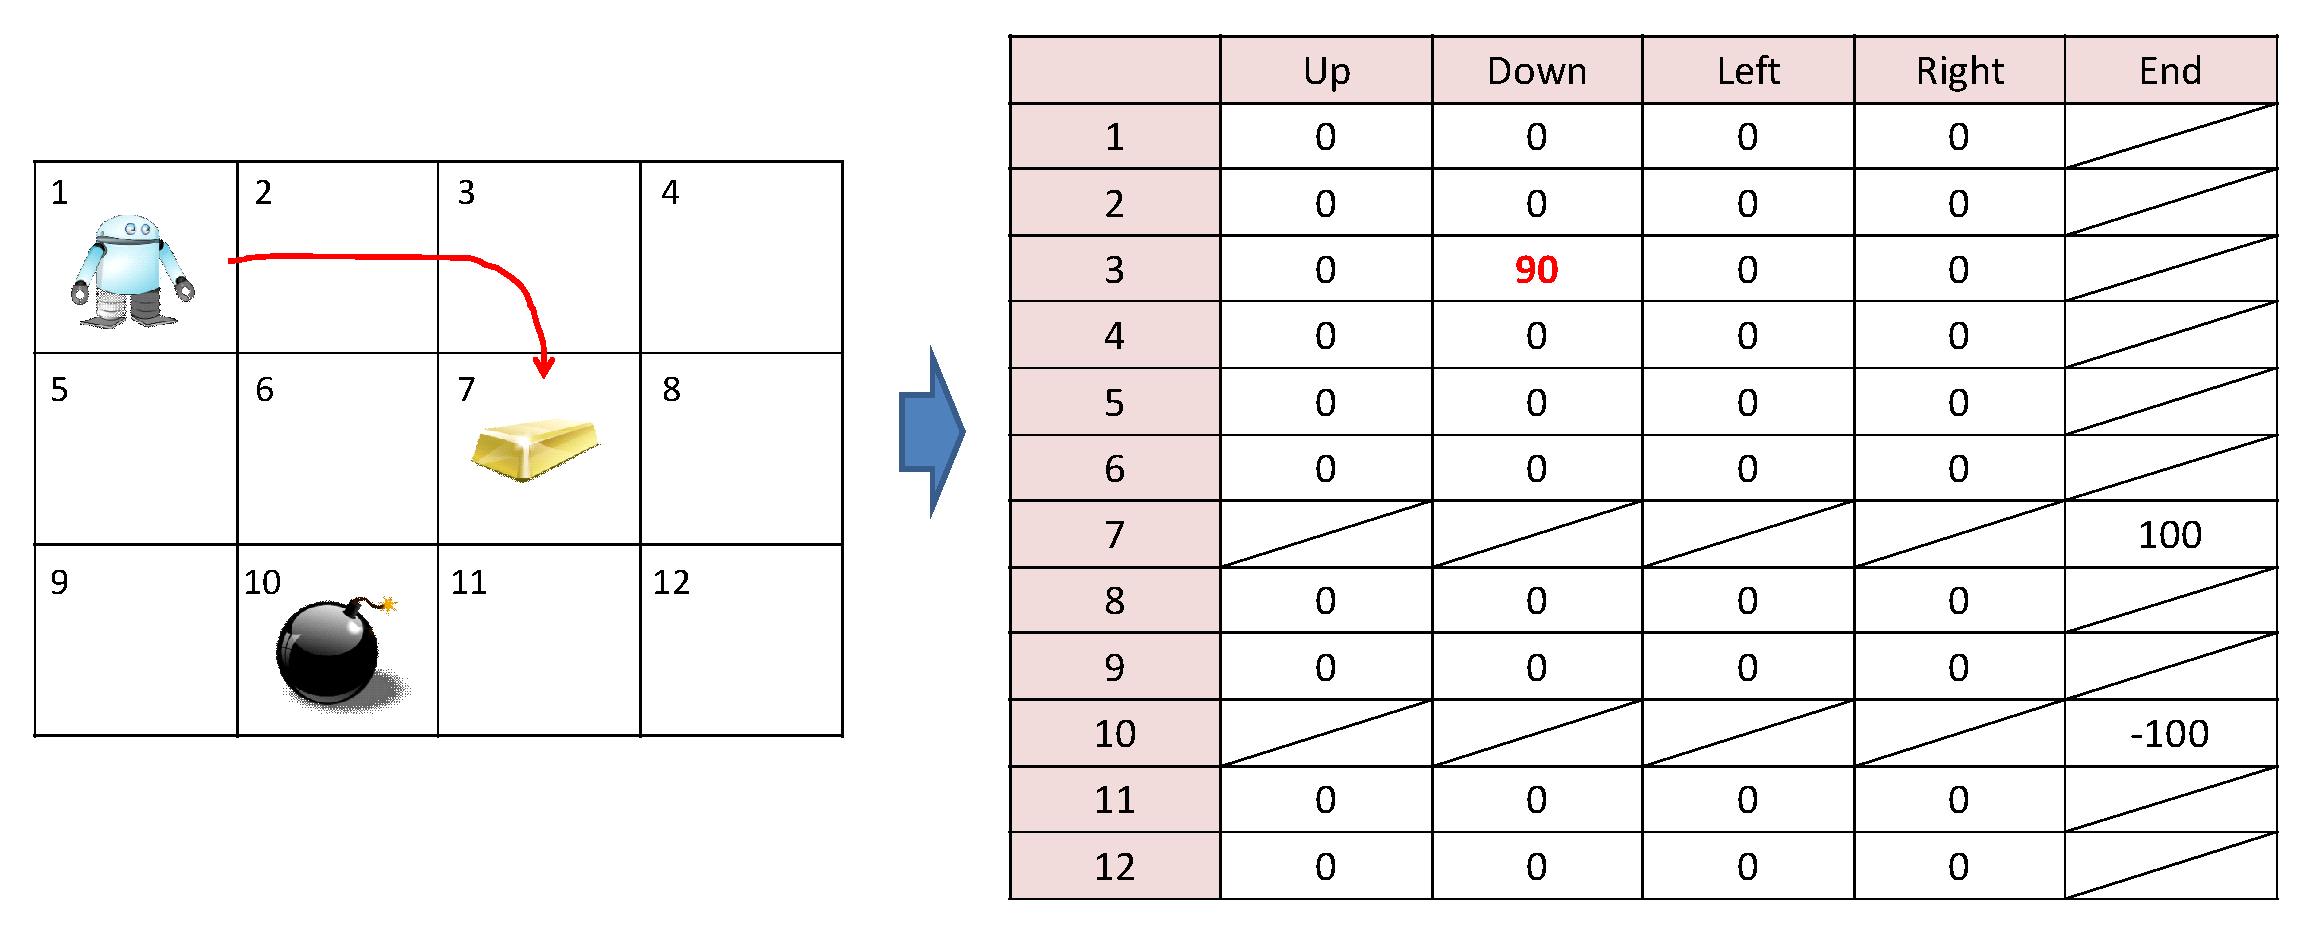
\includegraphics[width=140mm]{images/TsuruokaLab/ql3.eps}
 \end{center}
 \caption{Q学習(状態3から状態7に遷移した後)}
 \label{fig:ql3}
\end{figure}


\section{関数近似によるQ学習}

前節で説明したQ学習では,$Q(s,a)$の値を格納するためにテーブル(配列)を利用した.状態の数が
少ない場合にはこのような方法で学習を行うことができるが,現実の問題に強化学習を適用しようと
する場合,テーブルを利用したQ学習は不可能な場合が多い.例えば,ビデオゲームの AI を強化学習
で作ることを考えてみよう.入力として,ビデオゲームの画面,すなわち多数のピクセルから構成される画
像の情報を考えた場合,それによって決まる「状態」は無数に存在することになる.状態の数が非常に
大きい場合,テーブルに必要なメモリが莫大になることもさることながら,そもそもエージェントが同じ状態
を経験すること自体がまれになるため,学習が実質的にほとんど進まない.

関数近似 (function approximation) によるアプローチでは,$Q(s,a)$ をテーブルで表現するのではなく,
ニューラルネットワーク等,
パラメータ $\boldsymbol{\theta}$ によって規定される関数 $Q(s,a; \boldsymbol{\theta})$ で表現し,$Q^*(s,a)$ を精度
よく近似することを目指す.

いま,ある時点 $i$ でのパラメータを $\boldsymbol{\theta}_i$ としたとき,それをより適切
な値にするにはどのように更新すればよいだろうか? テーブルを用いたQ学習では,
$Q(s_t, a_t)$ を $r_{t+1} + \gamma \max_a Q(s_{t+1},a)$ に近づけるように更新を行ったのであった.
関数近似でも,それと同様の考え方により, $Q(s,a; \boldsymbol{\theta})$ を近づける目標として,
パラメータ $\boldsymbol{\theta}_{i-1}$ から計算される
\begin{equation}
y_i = r + \gamma \max_{a'} Q(s', a'; \boldsymbol{\theta}_{i-1})
\end{equation}
 を考え,それに対する
誤差が小さくするように更新を行うという方法が考えられる.誤差の基準として
2乗誤差を用いた場合は, 
\begin{equation}
L(\boldsymbol{\theta}_i) =  \mathbb{E}[ (y_i - Q(s,a; \boldsymbol{\theta}_i))^2 ]
\end{equation}
を最小化するようにパラメータを最適化する問題だとして解くことができる.

%関数近似に非線形関数であるニューラルネットワークを用いた手法として,Deep Q-Network 
%\cite{mnih2015humanlevel} がよく知られている.



\newpage
%!TEX root = ../main.tex
 \section{強化学習の実践}

 本節では,強化学習を用いて問題を解くAIを作成する方法を学ぶ.

 まず最初に,与えられた単純な迷路に対して報酬を最大化するAIを,単純なQ学習を用いて作ることで,強化学習の基礎を理解する.その後に,ChainerRLを用いて実践的なAIを作り,複雑な問題に対して強化学習を適用する方法を学ぶ.

  \subsection{準備}

  最初のタスクは,単純な迷路である.図\ref{fig:env1}に示す2次元の離散的な空間(グリッドワールド)において,スタートからゴールを目指すことが目標となる.図\ref{fig:env1}において,エージェントはSと書かれた位置($(y, x) = (0, 0)$)から行動を始め,Gと書かれた位置($(y, x) = (2, 3)$)にたどり着くことを目指す.エージェントは4方向に動くことができるが,灰色で表されるマスには侵入できない(移動できず1stepが経過する).エージェントは迷路全体を観測することはできず,自分のいる$x, y$座標を観測することができる.

  \begin{figure}[htb]
   \centering
   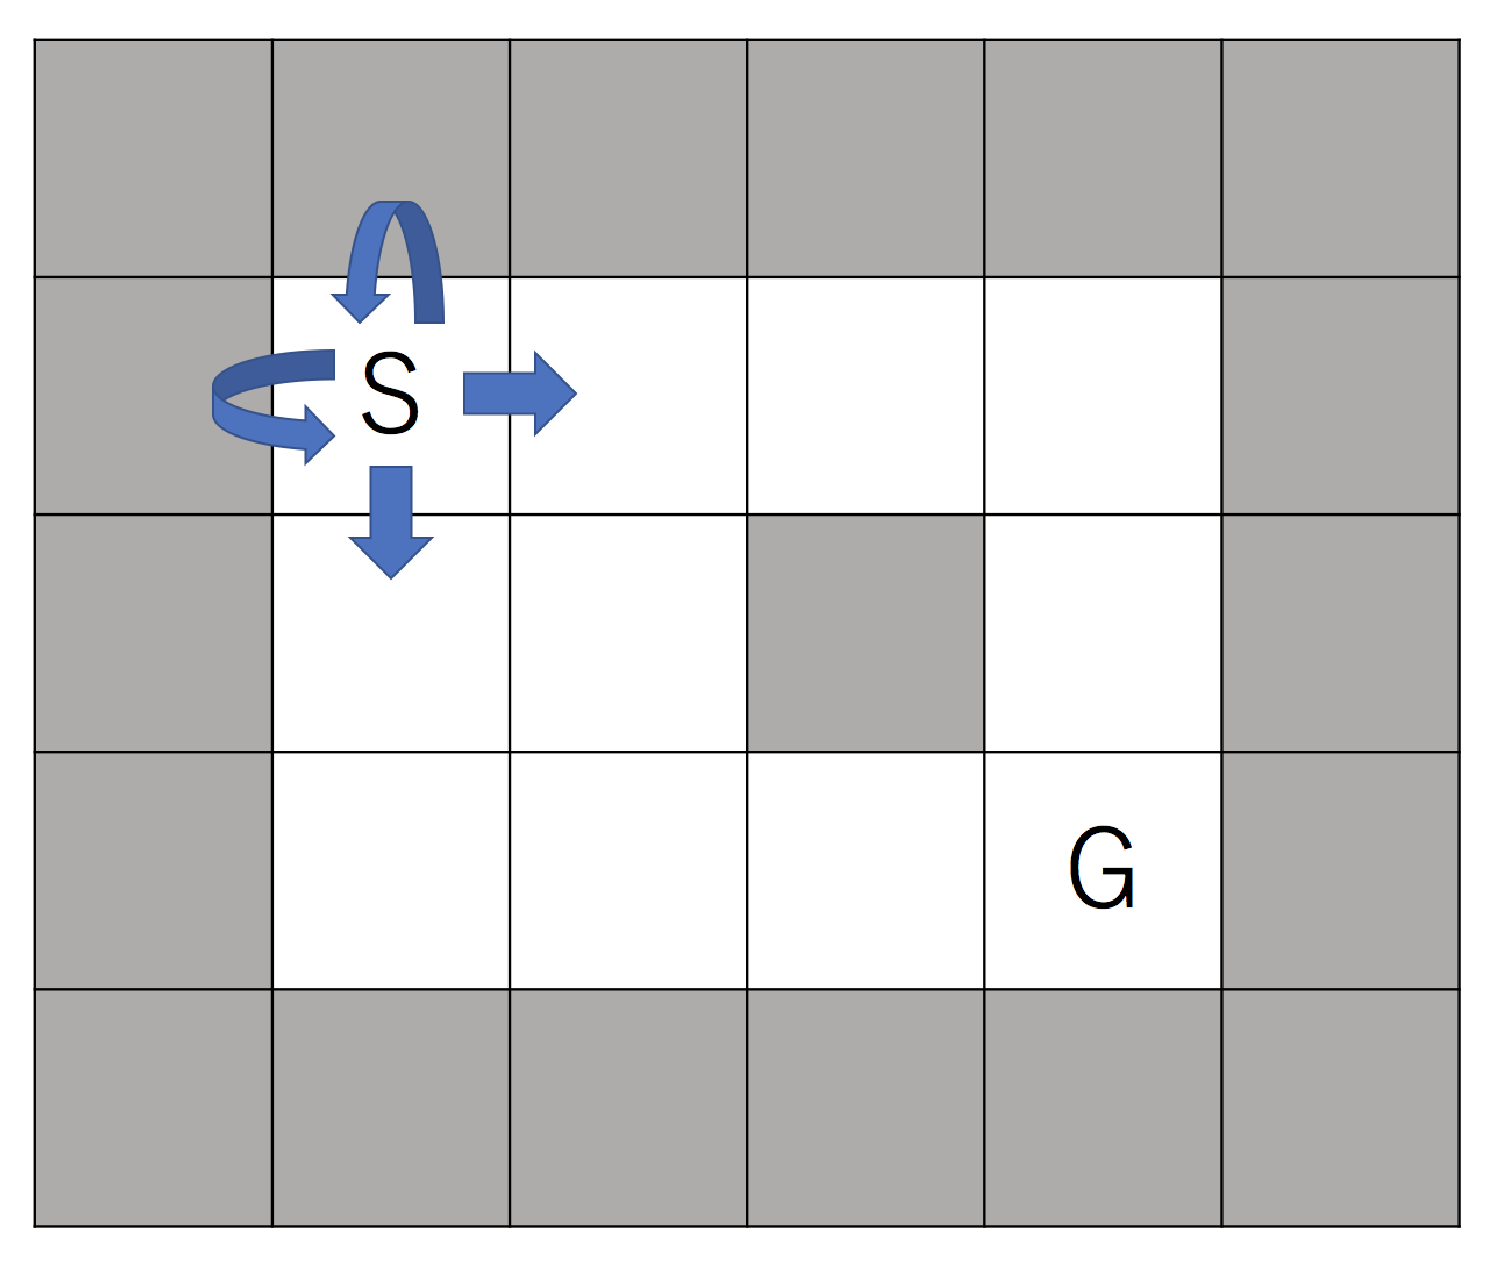
\includegraphics[width=80mm]{images/TsuruokaLab/env1.eps}
   \caption{単純な迷路}
   \label{fig:env1}
  \end{figure}

  \verb+dl_exp_rl.tar.gz+を展開してソースコードを入手しよう.ソースコードの中にある\verb+main.py+を実行することで,ランダムに動くエージェントが迷路に取り組む様子が観察できる.

  \newpage

   %$wget --http-user=dlexp --http-passwd=dlexp http://www.logos.ic.i.u-tokyo.ac.jp/~kkawamura/dl_exp/dl_exp_rl.tar.gz
  \begin{lstlisting}[basicstyle=\ttfamily\footnotesize, frame=single]
   $tar xzvf dl_exp_rl.tar.gz
   $cd dl_exp_rl
   $python main.py
  \end{lstlisting}


  \begin{practice}
   ソースコードをダウンロードし,\verb+main.py+を実行せよ.
   また,\verb+README.md+を読み,\verb+random_agent.py+ と \verb+easymaze_env.py+ の場所を確認せよ.
  \end{practice}

  迷路の様子が標準出力に一気に流れ込んでくるので,少し眺めたら\verb-Ctrl+c-で止めてしまって構わない.
  また,ゆっくり眺めたければ
  \begin{lstlisting}[basicstyle=\ttfamily\footnotesize, frame=single]
   $python main.py | less
  \end{lstlisting}
  のようにすればよい.

  \subsection{相互作用の理解}
  このタスクに限らず,強化学習は環境とエージェントが相互作用することで学習を行うものである.

  今回用いるソースコードは,オープンソースライブラリであるOpenAI Gym (\url{https://github.com/openai/gym}) ,およびChainerRL (\url{https://github.com/chainer/chainerrl}) の書式に則って書かれており,環境とエージェントが完全に分かれている.その二者の相互作用を担うのが\verb+main.py+である.

  \verb+main.py+を読み,適宜編集・実行しつつ,エージェントと環境がどのように相互作用しているのかを理解しよう.

  \begin{practice}
   \verb+main.py+の中で,envおよびagentを作成している行を答えよ.
   また,これらに対して呼び出されているインスタンス変数・メソッドをすべて挙げよ.
   自由課題などでenvやagentを自分で作成する場合,最低限これらの変数・メソッドをすべて実装する必要がある(インタフェース).
  \end{practice}

  演習の解答は\verb+answer_sheet.md+に書き込むとよい.

  なお,\verb+main.py+内の\verb+prints_detail+変数を\verb+False+にすることで,毎stepの迷路の出力を止めることができる.

  \begin{practice}
   \label{practice:100episodes}
   train, testのそれぞれで100 episodes の実験を行って,ランダムエージェントがゴールするまでのepisodeごとの平均step数を出力せよ.\verb+main.py+の編集が必要となる.
   300 steps 掛かってもゴールできない場合,300 steps でゴールしたものとして平均を計算せよ.
  \end{practice}

  episodeごとの平均rewardは既に出力されるようになっているので,その実装を参考にするとよい.

  \subsection{エージェントの理解}
  \label{subsec:rulebase}
  \verb+random_agent.py+を読み,ランダムエージェントがどのように動作しているかを理解しよう.

  ランダムエージェントは,\verb+__init__()+で行動集合のサイズを取得し,\verb+act()+が呼び出されると行動の中から一つをランダムに選ぶようになっている.

  ランダムエージェントはこの小さな迷路でもゴールするのにかなり時間がかかってしまうが,迷路の形状は毎回同じなので,人間であればすぐに最短経路を求めることができるはずである.

  例えば,「壁にぶつかるまで下に行き,ぶつかったら右に行く」などはその一例である.

  \begin{practice}
   \label{practice:rulebase}
   コメントを参考に,穴あきファイル\verb+rulebase_agent.py+の穴を埋めることで,この形状の迷路を最短step数で解くルールベースエージェントを作成せよ.「壁にぶつかるまで下に行き,ぶつかったら右に行く」ように実装すればよい.
   エージェントが受け取る観測を,\verb+print()+関数を用いたり\verb+easymaze_env.py+を読んだりすることで確認することが必要となることに注意せよ.
  \end{practice}

  \verb+main.py+の
  \begin{lstlisting}[basicstyle=\ttfamily\footnotesize, frame=single]
   agent = agents.RandomAgent(env, gpu_id)
  \end{lstlisting}
  を
  \begin{lstlisting}[basicstyle=\ttfamily\footnotesize, frame=single]
   agent = agents.RulebaseAgent(env, gpu_id)
  \end{lstlisting}
  に変更するだけで,ランダムエージェントの代わりにルールベースエージェントを試すことができる.

  また,\verb+rulebase_agent.py+内の
  \begin{lstlisting}[basicstyle=\ttfamily\footnotesize, frame=single]
   raise NotImplementedError()
  \end{lstlisting}
  は,「このセクションはまだ実装されていないので,ここを通るときは必ず実行時エラーを出してください」という合図である.穴を埋めた後はこの行を削除すればよい.


  \subsection{環境の理解}
  演習\ref{practice:rulebase}で作成したように,人間が迷路を観察し,あらかじめ移動ルールを定めておくことで,単純な迷路を解くAIは作成できる.

  しかしながら,この方法では異なる環境に対応できない.\verb+easymaze_env.py+を編集し,これを示そう.

  \begin{practice}
   \verb+easymaze_env.py+を編集し,迷路に最小限の変更を行うことで,演習\ref{practice:rulebase}で作成したエージェントがゴールできないような環境にせよ.ただし,別のルートでゴールできるようにしておくこと.
  \end{practice}

  この章ではあまり詳しく触れないが,自由課題で自作の環境に対して強化学習を適用したい場合,このソースコードを基に各メソッドを定義するとよい.特に\verb+_+から始まっているメソッドは必ず実装しなければならないものとなっている.

  \begin{practice}
   \verb+easymaze_env.py+において,\verb+_+から始まるメソッドをすべて探し出し,それぞれの役割を\verb+easymaze_env.py+に1行のコメントで書き込め.
  \end{practice}

  \subsection{Table Q学習の実装}
  Q学習は「ある状態からある行動を取ったとき,最大でいくら累積報酬がもらえるか」を学習する手法である.

  Q値のハッシュテーブルを用いて学習を行うエージェントを作成し,この迷路に適用してみよう.

  \begin{practice}
   コメントを参考に,穴あきファイル\verb+table_q_agent.py+の穴を埋めることで,table-Q エージェントを実装せよ.
   ルールベースエージェントの代わりにtable-Q エージェントを用いるために,\verb+main.py+も変更する必要があることに注意せよ.
  \end{practice}

  \begin{practice}
   演習\ref{practice:100episodes}と同様に,100 episodes の実験を行って,table-Q エージェントがゴールするまでの平均step数を出力せよ.
   また,trainのうち,最初の10 episodes,最後の10 episodesの平均step数を出力せよ.
  \end{practice}

  \begin{practice}
   table-Q エージェントには,迷路の各地点におけるQ値を文字列形式で出力する\verb+q_table_to_str()+メソッドが用意されている.このメソッドを適宜呼び出し\verb+print()+することで,Q値が学習されていく過程を観察せよ.時間があれば,割引率や学習率,迷路の報酬などを変えて,学習の過程がどのように変わるかを観察してみよ.
  \end{practice}

  \subsection{TrainとTest,On-PolicyとOff-Policy}
  教師あり学習においてtrainデータとtestデータが区別されるように,強化学習においてもtrainとtestという概念がある.

  強化学習では,エージェントは方策 (policy) $\pi$を持っており,環境から得られた観測$s$に対して行動集合上の確率分布$\pi(s)$に従って行動$a\sim \pi(s)$を選択する.
  train時の行動選択に用いる方策$\pi$について,その方策$\pi$をより良い方策にしていく学習を方策オン型 (on-policy) という.これに対し,$\pi$とは別のtest時用の方策$\pi'$を用意し,この方策$\pi'$を最適方策に近づけていく学習を方策オフ型 (off-policy) という~\cite{david2017policy}.

  方策オフ型学習の利点の一つとして,強化学習において大きな問題の一つである探索と活用の問題を避けることができる点が挙げられる.
  強化学習においては,次の行動を選択する際に,「これまでの学習によって,既に良いとわかっている行動」を取るべきか,「これまでの学習で,まだ良いか悪いか判断できない行動」を取るべきか,という問題に直面することになる.前者だけを取っていては局所解に陥ってしまい,後者だけを取っていては報酬を最大化することができない.前者を取ることを活用 (exploitation),後者を取ることを探索 (exploration)という.
  方策オフ型学習では,少なくともtest時にはこの問題を回避することができる.test時には探索は不要だからである.

  Q学習における$\varepsilon$-greedyは,この探索と活用の問題を解決するための手法の一つである.train時において,Q学習エージェントはできるだけQ値の高い行動を選択することで,現時点で「良い」と思われる行動についてより多く学習したい(活用).しかしながら,活用だけでは「まだ見つかっていない」より良い行動を学習することができない(探索).そこで,一定の確率でランダムに行動し ($\varepsilon$),それ以外のときQ値が最大の行動を選択することを考える (greedy).このようにすることで,探索と活用を両立することができる.

  Q学習は方策オフ型の学習である.なぜなら,train時にのみ$\varepsilon$-greedyを用いて学習し,test時は常にQ値が最大の行動を選択するからである.
  この意味で,前項で実装したtable-Q エージェントはQ学習の実装としては十分はでない.これを修正しよう.

  \begin{practice}
   Table-Q エージェントを,train時に$\varepsilon$-greedyで行動し,test時にgreedyで行動するようにせよ.
   その後,演習\ref{practice:100episodes}と同様に,100 episodes の実験を行って,エージェントがゴールするまでの平均step数を出力し,train時とtest時の結果を比較せよ.
  \end{practice}

  実装の仕方がわからない場合は,まずtrain時とtest時で行動を選択するときにどのメソッドが呼び出されるかに着目してみよ.
  $\varepsilon$-greedy自体は既に\verb+table_q_agent.py+に実装されているはずである.train時にはこれを行い,test時にはgreedyに行動するようにすればよい.

  ただし,\verb+main.py+を書き換えて呼び出すメソッドを変えてはいけない.エージェントのインタフェースは共通のものを用いているからである.

  正しく実装できていれば,test時には第\ref{subsec:rulebase}項で実装したルールベースエージェントと同じ最短距離でゴールすることができるはずである.

  \subsection{Deep Q-Network}
  ここまでで我々は,ハッシュテーブルを用いて実装されたQ学習が,単純な環境に対して最適方策を学習できることを見てきた.しかしながら,この方法は環境が複雑になると適用できなくなってしまう.

  例えば,環境の状態$s$が離散的な値ではなく連続量になることを考えてみよう.今回の実装では$Q(s, a)$は$s$をキーとするdictionary (hash)で実装されており,$s$が連続量になると同じ状態が起こる確率がほぼ0になってしまうため,学習ができなくなってしまう.また,$s$が離散値であっても,空間がメモリに乗り切らないほど大きければ,やはり今回の実装では学習ができなくなってしまう.

  このような環境に対処するために,$Q(s, a)$をハッシュテーブルではなくニューラルネットワークを用いて表現することを考える.すなわち,Q関数を連続量を取る関数で近似することで,環境の状態が連続量であっても対処できるようにする.ニューラルネットワークはweightの次元数を(学習対象と無関係に)自由に定めることができるので,環境の状態数が非常に大きかったとしても,(正しく学習できる保証はないが)メモリに乗り切る程度のweightでQ関数を表現することができる.

  Q学習をニューラルネットワークを用いて行う方法を考えよう.通常のQ学習では,状態$s$に対して行動$a$を取り,報酬$r$と次状態$s'$を得た場合の更新式は次のようになる.
  \begin{equation}
   Q(s, a) \leftarrow Q(s, a) + \alpha \left( r + \gamma \max_{a'} Q(s', a') - Q(s, a)\right)
  \end{equation}
  Q学習が十分収束したとき,この更新式を用いても$Q$は更新されないはずである.すなわち,
  \begin{equation}
    r + \gamma \max_{a'} Q(s', a') - Q(s, a) \simeq 0
  \end{equation}
  となっているはずである.実際,この式が成立しているということは,Q値が「現状態における報酬と,次状態以降の累積報酬の最大値の和」を表しているということであるから,Q値を正しく学習できているということになる.

  すなわち,Q学習とは,大量の学習データ$(s, a, r, s')$に対して,
  \begin{equation}
   \label{eq:QNetEq}
   Q(s, a) = r + \gamma \max_{a'} Q(s', a')
  \end{equation}
  が成り立つような関数$Q$を求める学習であるといえる.これは教師あり学習と同様であるから,二乗誤差などを用いて左辺と右辺の差を最小化するようにニューラルネットワークを学習させればよい.

  Mnihらが2015年に発表したdeep Q-network (DQN) では,この基本アイディア以外に様々な工夫が為されている.例えば以下のようなものである:
  \begin{itemize}
   \item Experience replay.学習データをreplay bufferと呼ばれるバッファに溜め込み,そこからランダムにサンプリングして学習を行う.これにより,学習データの時間的相関を減らすことができ,学習が安定する.
   \item Fixed target Q-network.学習対象となる式(\ref{eq:QNetEq})の左辺に用いられるQ関数を固定し,一定時間ごとに最新のQ関数に置き換える.これにより,学習対象があまり変化しなくなり,学習が安定する.
  \end{itemize}

  ChainerRLを用いると,DQNを始めとする様々な深層強化学習の手法を手軽に実装することができる.これを確かめよう.

  \begin{practice}
   \verb+main.py+を編集し,DQN エージェント (\verb+agents/dqn_agent.py+) にこの迷路を解かせてみよ.
   その後,\verb+dqn_agent.py+,\verb+agents/models/dqn_models.py+を読んでみよ.重要な実装はすべてchainerrlが担当していて,最小限の記述でDQNが実装できていることがわかるはずである.
   時間があれば,DQNのモデルを色々変えて(線形回帰にしてみる,活性化関数を変えてみるなど),学習がどのように変わるかを観察せよ.
  \end{practice}

  \subsection{状態空間が連続な環境におけるQ学習}

  前項で述べたとおり,ハッシュテーブルを用いて実装したQ学習では,環境の状態が連続値になったときに対応できない.
  これに対して,DQNでは,Q関数をニューラルネットワークを用いて表現しているため,状態空間が連続になっても対応できる.
  これを確かめよう.

  \subsubsection{CartPole}

  状態空間が連続なゲームとして,ここではOpenAI Gymに実装されているCartPoleというゲームを扱う.

  CartPoleは次のようなゲームである.まず,図\ref{fig:cartpole}のように黒い台車の上に茶色の棒が乗った状況を考える.棒の下端は台車に取り付けられており,放っておくと棒は下端を中心に回転してしまう.エージェントは台車を右または左のどちらかに押すことができる.この状況で,できるだけ長い間棒を倒さないようにすることが目標となる.観測として台車の位置,速度,棒の角度,角速度の4つの実数が与えられ,ゲームが終了していなければエージェントは各stepで1単位の報酬を得る.エージェントが行える行動は右に押すか,左に押すかの2択のみである.棒が一定以上傾くか,台車が一定範囲外に出るか,200steps が経過した時点でゲームは終了する.すなわち,報酬の最大値は200である.

  \begin{figure}[htb]
   \centering
   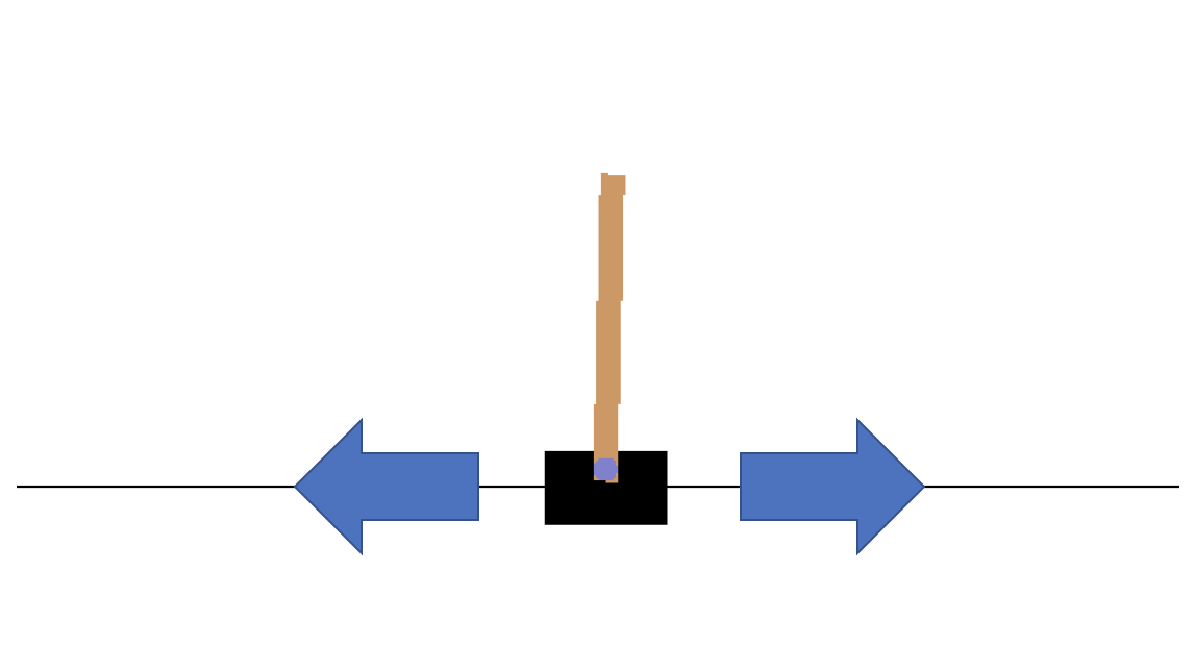
\includegraphics[width=80mm]{images/TsuruokaLab/cartpole.eps}
   \caption{Cart Pole の様子}
   \label{fig:cartpole}
  \end{figure}

  \verb+main.py+の
  \begin{lstlisting}[basicstyle=\ttfamily\footnotesize, frame=single]
   env = gym.make('Easymaze-v0')
  \end{lstlisting}
  を
  \begin{lstlisting}[basicstyle=\ttfamily\footnotesize, frame=single]
   env = gym.make('CartPole-v0')
  \end{lstlisting}
  に変更するだけで,CartPoleを試すことができる.

  \begin{practice}
   CartPoleに対してDQNを学習させ,様子を観察せよ.もし余裕があれば,ローカル環境(学科PCなど)でも試してみるとよい.ローカル環境では,\verb+main.py+の\verb+prints_detail+変数を\verb+True+にすることで,エージェントがCartPoleをプレイする様子を動画で見ることができる.
   ゲームは棒が15度傾いた時点で終わってしまうので,各episodeが一瞬で終わってしまって動画がよくわからないかもしれない.その場合は,\verb+done+が\verb+True+になってもループを抜けずに\verb+env.render()+を続けるようにするとよい.
  \end{practice}

  先述の通り,報酬の最大値は200点である.おそらく,現在のDQNは数十点程度しか取れなかったことだろう.

  \begin{practice}
   CartPoleにおいて,10episodes連続で200点を取ることができるエージェントを作成せよ.
   現在のDQNのどこに問題があるのかを考え・調べ,様々な方法を試してみよ.
  \end{practice}

  例えば,以下のような項目を調べるとよい.
  \begin{itemize}
   \item 隠れ層の大きさや枚数は必要十分か.
   \item 学習率や最適化アルゴリズムは適切か.
   \item 学習のepisode数は十分か.
   \item 過学習を起こしていないか.
   \item 探索の方式は適切か.
   \item Replay bufferは小さすぎないか.
   \item DQNより良いアルゴリズムはないか.
  \end{itemize}

  周りの学生やTAと相談し,できるだけ高得点を取ることのできるエージェントを作ろう.

  \subsection{発展課題・アイディア}

  ここでは,実験後半の自由課題で強化学習を使いたい学生のために,いくつか課題の種を挙げる.これらの課題のうちいずれかを選択してもよいし,これらを基に自由に課題を設定してもらっても構わない.

  \begin{itemize}
   \item OpenAI Gym には,様々なゲームが用意されている.CartPoleのように比較的単純なゲームだけでなく,ビデオゲーム(Atari)や対戦ゲーム(囲碁)などもある.これらのゲームで高得点を得られるエージェントを作ってみよう.その際,1つのゲームに特化するのか,どんなゲームにも適用できるようにするのかは意識するべきである.例えば,今年の6月にはMicrosoftのチームがAtariの ``Ms. Pac-Man''で最高得点である999,990点を取ったと発表した~\cite{allison2017pacman}が,彼らはこのゲームに特化したエージェントを作っており,全く事前知識を用いていないというわけではない.その一方で,DeepMindが発表したDQNは,Atariの49のゲーム全てに全く同じパラメータを用いて学習させ,多くのゲームで人間を超えるスコアを出しているが,すべてのゲームで最高得点を取ったというわけではない.
   \item 強化学習は非常に一般的なモデルであり,現実の様々な問題に適用できるはずである.解決すべき身近な問題を見つけ,強化学習の仕組みに落とし込むことで解決してみよう.制御・最適化などの分野や,自律ロボットの行動などが応用先として有名である.
   \item この実験の他のトピックと組み合わせてみよう.画像分類で強化学習をするとはどういうことだろうか? あるいは,翻訳や要約と強化学習を組み合わせるとどうなるだろうか?
   \item 最新の強化学習の手法を調べ,実装してみよう.まだソースコードが公開されていないなら,実装して世界に公開することで,誰かの役に立てるかもしれない.
   \item ソーシャルゲームや有名なボードゲームなど,身近なゲームを\verb+gym.Env+として実装し,強化学習を適用してみよう.どのようなエージェントが得られるだろうか.
   \item 強化学習の手法を,他の手法と比較してみよう.例えば,強化学習の環境として仮定されているMarkov Decision Processでは,状態遷移規則$T(s, a)\in S$がわかっていれば線形計画法などで解くことができる.また,遺伝的アルゴリズムなどを用いてもエージェントを作ることができる.これらの手法と強化学習の手法との違いはなんだろうか.
   \item 強化学習のエージェントが取れる点数をゲームの「難しさ」だと考えることで,ゲームの難易度調整をしてみよう.例えば,プレイしているうちにだんだんと難易度がユーザにとって最適なものになっていくゲームが作れないだろうか?
   \item 2017年10月19日にGoogle DeepMindが強化学習で(人間の棋譜を用いずに)囲碁の強いエージェントを作ることに成功したと発表した (\url{https://deepmind.com/blog/alphago-zero-learning-scratch/}).この論文を読み,AlphaGo Zeroがどのようにして学習を行っているのかを理解し,まとめてみよう.OpenAI Gymの枠組みでAlphaGo Zeroは実装できるだろうか? もしできないとしたら,それはなぜか?
  \end{itemize}


% 画像認識部分
\chapter{Image Recognition}
%!TEX root = ../main.tex

\section{CNNとは}
主に全結合層,畳み込み層,プーリング層から構成されるDeep Neural Networks (DNN) のことである.各層はニューロンによって構成される.

\subsection{全結合層}
全結合層 (FC層) に含まれる各ニューロンは前の層の全てのニューロンと連結している.前の層の出力を\(h^{i-1}\)とすると重み\(W\)のFC層の出力\(h^i\)は
\[
h^i = Wh^{i-1} + b.
\]
\(b\)は定数である.下の図\ref{fig:fc1}と\ref{fig:fc2}はそれぞれFC層の構造とどのようにニューロンの値を計算するかを示したものである.定数bも学習対象ではあるが省略している.

\begin{figure}[ht]
    \begin{tabular}{cc}
      %---- 最初の図 ---------------------------
      \begin{minipage}[t]{0.4\hsize}
        \centering
        \includegraphics[width=0.95\linewidth]{images/YamasakiLab/sec1/fc1.eps}
        \caption{FC層の構造}
        \label{fig:fc1}
      \end{minipage} &
      %---- 2番目の図 --------------------------
      \begin{minipage}[t]{0.6\hsize}
        \centering
        \includegraphics[width=0.95\linewidth]{images/YamasakiLab/sec1/fc2.eps}
        \caption{FC層の計算と学習対象}
        \label{fig:fc2}
      \end{minipage}
      %---- 図はここまで ----------------------
    \end{tabular}
  \end{figure}


\subsection{畳み込み層}
畳み込み層はカーネルと呼ばれる小さな受容野をもとに結合していくため前層のニューロンに対して疎結合となる.これは局所特徴に注目することに相当する.
言葉で説明すると分かりづらいが図~\ref{fig:conv1}と図~\ref{fig:conv2}を見てほしい.
いくつかのkernelを畳み込むことで新しい層を作っている.第i層のサイズは第i-1層のサイズとpadding,kernelのサイズとstride幅によって決まる.paddingというのは第i-1層の周囲に適当な数字をくっつけてサイズを大きくするためのものである.kernelのサイズは縦と横の大きさのことであり,チャンネル(厚み)は第i-1層と同じである.
stride幅は畳み込む時にkernelを移動させる幅のことを意味し,大きければ大きいほど第i層のサイズは小さくなる.

また第i層の厚み,すなわちチャンネル数はkernelの数と等しい.これは図~\ref{fig:conv1}と~\ref{fig:conv2}をじっくり見比べてもらえばわかると思う.

\begin{figure}[ht]
	\begin{center}
		\includegraphics[width=0.7\linewidth] {images/YamasakiLab/sec1/conv1.eps}
		\caption{畳み込み層の構造}
		\label{fig:conv1}
	\end{center}
\end{figure}
\begin{figure}[ht]
	\begin{center}
		\includegraphics[width=0.7\linewidth] {images/YamasakiLab/sec1/conv2.eps}
		\caption{畳み込み層の計算と学習対象}
		\label{fig:conv2}
	\end{center}
\end{figure}

\subsection{プーリング層}
畳み込み層と似ているがパラメータは固定されており,学習対象は存在しない.図~\ref{fig:pool1}はkernelが見ている範囲の平均値を出力するものである(average poolingと呼ばれる).

プーリング層の目的は画像内の特徴に関して,位置情報を曖昧にするためである.プーリングを行なうことで位置の変化に対して頑健な特徴表現を学習できる.平均値を求めるもの以外にも注目領域内の最大値を出力するmax poolingなどが存在する.

\begin{figure}[ht]
	\begin{center}
		\includegraphics[width=0.7\linewidth] {images/YamasakiLab/sec1/pool1.eps}
		\caption{プーリング層の計算}
		\label{fig:pool1}
	\end{center}
\end{figure}

\subsection{活性化関数}
FC層や畳み込み層は結局のところ線形変換であり,このままでは豊かな変換能力を習得できない (線形変換を重ね合わせたところで表現能力は増さない) ため,殆どの場合,各ニューロンに対して活性化関数を適用することで非線形変換を学習させる.図~\ref{fig:activate}はFC層に対して活性化関数を適用している図である.学習対象は何もないがこれにより非線形変換を表現できる.\(\phi\)にはsigmoid関数やReLU関数がよく用いられ,特に画像分野ではReLU関数が注目を集めている.

\begin{figure}[ht]
	\begin{center}
		\includegraphics[width=0.7\linewidth] {images/YamasakiLab/sec1/activate.eps}
		\caption{活性化関数}
		\label{fig:activate}
	\end{center}
\end{figure}

\subsection{畳み込み層と全結合層}
畳み込み層は1次元的なイメージなのに対し畳み込み層は3次元であるためその結合がイメージしづらいと思う.
そこで図~\ref{fig:conv_to_fc}を見てもらえればまだなんとなくなイメージがつかめるのではないだろうか.
図はchannel数3,高さ2,幅2の3次元の第$i-1$層からサイズ5のFC層への連結方法を示している.図が煩雑になるので第$i-1$層の1channel目からしか線を伸ばさなかったが要は全ニューロン同士が連結していることを掴んでもらえば問題ない.

\begin{figure}[ht]
	\begin{center}
		\includegraphics[width=0.7\linewidth] {images/YamasakiLab/sec1/conv_to_fc.eps}
		\caption{畳み込み層から全結合層へ}
		\label{fig:conv_to_fc}
	\end{center}
\end{figure}


以上のことは
\url{https://qiita.com/icoxfog417/items/5fd55fad152231d706c2}や\url{https://deepage.net/deep_learning/2016/11/07/convolutional_neural_network.html}により,詳細に説明されている.
上記以外にもDropOutやBatch Normalization等様々な手法が提案されている.調べてみたりTAに聞いてみたりしよう.

また有名なCNNであるVGG16やResNet等の構造を調べてみよう.
%!TEX root = ../main.tex

\section{chainerの基礎}
本章では,deeplearningのフレームワークの一つであるchainerについて基本的なコードを用いて説明する.
\subsection{開発環境について}
\subsubsection{sshについて}
配布したuser名,パスワードで以下のコマンドで開発環境にログインできる.

\begin{lstlisting}[basicstyle=\ttfamily\footnotesize, frame=single]
ssh Username@IPaddress
\end{lstlisting}
yes/noを聞かれるので,yesと入力した後,配られたパスワードを入力することでログインできる.

この工程を簡略化したい場合は,\url{https://qiita.com/ir-yk/items/af8550fea92b5c5f7fca},
\url{https://qiita.com/passol78/items/2ad123e39efeb1a5286b}などを参考にすること.
\subsubsection{scpについて}
コードを編集する際,リモートではなく,ローカルで編集しその結果をリモートに反映させたいという需要があると思う.
その際は,scpコマンドを用いる.
\begin{lstlisting}[basicstyle=\ttfamily\footnotesize, frame=single]
scp LocalFilePath Username@IP:RemotePath
\end{lstlisting}
と打てば,ローカル→リモートにファイルの転送ができる.その他の使い方については,\url{https://qiita.com/katsukii/items/225cd3de6d3d06a9abcb}などを参考にすること.

また,エディタによってはこういった機能をサポートしてくれるものもある.""使っているエディタ sftp""などで検索すると良い.

\subsubsection{tmuxについて}
開発環境でコードを実行していてもそのままだと,パソコンを閉じる,開発環境と接続を切るなどすると実行が終了してしまう.それを防ぐのがtmuxである.tmux上で実行すればこういった問題を解決できる.詳細については,
\url{https://qiita.com/vintersnow/items/be4b29652ff665c45198}などを参考にすること.
\subsection{サンプルコードの実行}
今回扱うサンプルコードはmnistと呼ばれる手書き数字の分類を行うものである.
\begin{practice}
train\_mnist\_mlp.pyをGPUで実行せよ.

次のコマンドを打つと学習を開始できる.
\begin{lstlisting}[basicstyle=\ttfamily\footnotesize, frame=single]
python train_mnist_mlp.py -g 0
\end{lstlisting}

\end{practice}
数分待つと,学習が終了し,resultフォルダに結果が出力されている.
\begin{figure}[ht]
	\begin{center}
		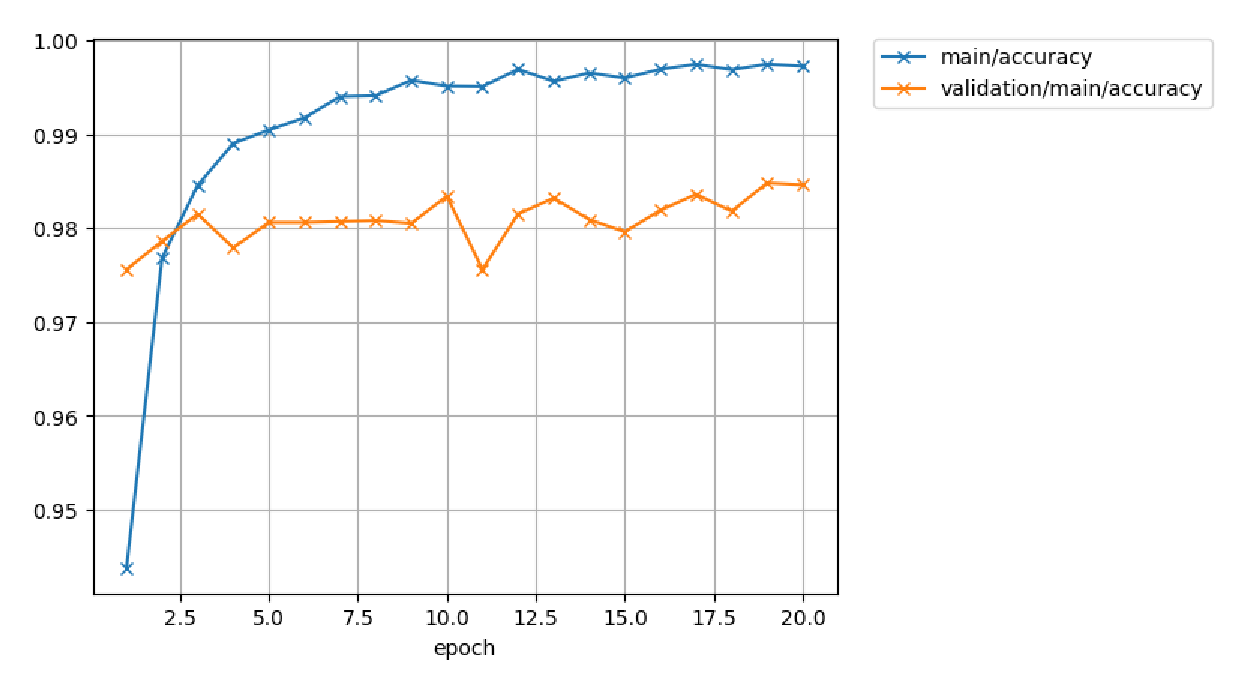
\includegraphics[width=0.7\linewidth] {images/YamasakiLab/sec2/accuracy.eps}
		\caption{学習結果の例}
		\label{fig:accuracy}
	\end{center}
\end{figure}


次に,学習がうまくできたか確認する.
\begin{practice}
白黒の手書き数字画像を作成せよ.
この時黒地に白文字で数字を書くことに注意する.(学習させた手書き数字データが黒地に白なので)
\end{practice}

\begin{figure}[ht]
	\begin{center}
		\includegraphics[width=0.2\linewidth] {images/YamasakiLab/sec2/number.eps}
		\caption{手書き数字の例}
		\label{fig:num}
	\end{center}
\end{figure}

\begin{practice}
自分が書いた手書き文字を先程学習したモデルに通して出力を表示し,正しく数字が認識されたか確かめよ.
次のコマンドでテストコードを実行できる.
\begin{lstlisting}[basicstyle=\ttfamily\footnotesize, frame=single]
python test_mnist_mlp.py -g 0 -i (path to the input image) -m result/model_20
\end{lstlisting}

\end{practice}

\subsection{サンプルコードの解説}
先の章で実行したサンプルコードについて簡単に解説を行う.
chainerの公式ドキュメント(https://docs.chainer.org/en/stable/)を適宜参考にすること.

\subsubsection{コマンドライン引数}
% \pythonexternal{YamasakiLab/code/sec2_command.py}
\begin{lstlisting}[basicstyle=\ttfamily\footnotesize, frame=single]
    parser = argparse.ArgumentParser(description=‘Chainer example: MNIST’)
    parser.add_argument(‘--batchsize’, ‘-b’, type=int, default=100,
                        help=‘Number of images in each mini-batch’)
    parser.add_argument(‘--epoch’, ‘-e’, type=int, default=20,
                        help=‘Number of sweeps over the dataset to train’)
    parser.add_argument(‘--frequency’, ‘-f’, type=int, default=-1,
                        help=‘Frequency of taking a snapshot’)
    parser.add_argument(‘--gpu’, ‘-g’, type=int, default=-1,
                        help=‘GPU ID (negative value indicates CPU)‘)
    parser.add_argument(‘--out’, ‘-o’, default=‘result’,
                        help=‘Directory to output the result’)
    parser.add_argument(‘--resume’, ‘-r’, default=‘’,
                        help=‘Resume the training from snapshot’)
    parser.add_argument(‘--unit’, ‘-u’, type=int, default=1000,
                        help=‘Number of units’)
    args = parser.parse_args()
\end{lstlisting}
このプログラムで使うことのできるコマンドライン引数を定義している.各変数に対する説明は省略する.

\subsubsection{モデル}
% \pythonexternal{YamasakiLab/code/sec2_mlp.py}
\begin{lstlisting}[basicstyle=\ttfamily\footnotesize, frame=single]
 model = MLP(args.unit, 10)
     if args.gpu >= 0:
        # Make a specified GPU current
        chainer.cuda.get_device_from_id(args.gpu).use()
        model.to_gpu()  # Copy the model to the GPU
\end{lstlisting}
この行で今回の学習に用いるモデルを定義している.また,GPUを使用していたらモデルをGPUに変更していいる.args.gpuは使用するGPUの番号を示している.
MLP自体は以下で定義している.
\begin{lstlisting}[basicstyle=\ttfamily\footnotesize, frame=single]
class MLP(chainer.Chain):
    def __init__(self, n_units, n_out):
        super(MLP, self).__init__()
        with self.init_scope():
            self.l1 = L.Linear(None, n_units)  # n_in -> n_units
            self.l2 = L.Linear(None, n_units)  # n_units -> n_units
            self.l3 = L.Linear(None, n_out)  # n_units -> n_out

    def __call__(self, x, t=None):
        h = F.relu(self.l1(x))
        h = F.relu(self.l2(h))
        h = self.l3(h)

        loss = F.softmax_cross_entropy(h, t)
        accuracy = F.accuracy(h, t)
        chainer.report({‘loss’: loss}, self)
        chainer.report({‘accuracy’: accuracy}, self)

        if chainer.config.train:
            return loss
        else:
            return h

    def predict(self, x):
        h = F.relu(self.l1(x))
        h = F.relu(self.l2(h))
        h = self.l3(h)
        return h
\end{lstlisting}

init関数で今回使うネットワークの構造を定義しており,今回は入力層(l1),中間層(l2),出力層(l3)の全3層である.今回用いた層は全て全結合層である.
xがネットワークのinput,hがネットワークのoutput,tがinputの正解ラベルである.trainの時はlossを返し学習をさせており,validationの時は学習をさせたくないのでhを返している.(validationの時も学習させてしまうとvalidationのaccuracyが正当な評価にならない.)

\subsubsection{optimizer}
\begin{lstlisting}[basicstyle=\ttfamily\footnotesize, frame=single]
    # Setup an optimizer
    optimizer = chainer.optimizers.Adam()
    optimizer.setup(model)
\end{lstlisting}
この部分では,lossを最適化するための手法を決めておりこのプログラムではAdamを用いている.
他の最適化手法を用いたい場合はhttps://docs.chainer.org/en/stable/reference/optimizers.htmlなどを参考にすること.

\subsubsection{データセット}
\begin{lstlisting}[basicstyle=\ttfamily\footnotesize, frame=single]
   # Load the MNIST dataset
    train, test = chainer.datasets.get_mnist()
\end{lstlisting}
この部分では,今回の学習に用いるデータセットを定義している.今回用いたmnistのデータセットはchainerが用意してくれているのでこのように1行書くだけで呼び出せる.自分で用意したデータセットを用いたい場合については後の演習に譲る.
 
 \subsubsection{Trainerの準備}
\begin{lstlisting}[basicstyle=\ttfamily\footnotesize, frame=single]
    train_iter = chainer.iterators.SerialIterator(train, args.batchsize)
    test_iter = chainer.iterators.SerialIterator(test, args.batchsize,
                                                 repeat=False, shuffle=False)

    # Set up a trainer
    updater = training.StandardUpdater(train_iter, optimizer, device=args.gpu)
    trainer = training.Trainer(updater, (args.epoch, ‘epoch’), out=args.out)
\end{lstlisting}
 これまでに定義したものを用いて学習のためのTrainerを作成している.
  \subsubsection{modelの評価と結果の可視化}
\begin{lstlisting}[basicstyle=\ttfamily\footnotesize, frame=single]
    # Evaluate the model with the test dataset for each epoch
    trainer.extend(extensions.Evaluator(test_iter, model, device=args.gpu))

    trainer.extend(extensions.dump_graph(‘main/loss’))

    frequency = args.epoch if args.frequency == -1 else max(1, args.frequency)
    trainer.extend(extensions.snapshot(), trigger=(frequency, ‘epoch’))
    trainer.extend(extensions.snapshot_object(model, ‘model_{.updater.epoch}’),
                   trigger=(frequency, ‘epoch’))


    trainer.extend(extensions.LogReport())
    if extensions.PlotReport.available():
        trainer.extend(
            extensions.PlotReport([‘main/loss’, ‘validation/main/loss’],
                                  ‘epoch’, file_name=‘loss.png’))
        trainer.extend(
            extensions.PlotReport(
                [‘main/accuracy’, ‘validation/main/accuracy’],
                ‘epoch’, file_name=‘accuracy.png’))

    trainer.extend(extensions.PrintReport(
        [‘epoch’, ‘main/loss’, ‘validation/main/loss’,
         ‘main/accuracy’, ‘validation/main/accuracy’, ‘elapsed_time’]))

    trainer.extend(extensions.ProgressBar())
\end{lstlisting}
ここでは,学習結果の出力と可視化を主に行なっている.extensions.snapshot\_object関数は,学習したモデルを出力する関数で,triggerはその出力を何epoch毎に行うかを決定している.他の関数については説明を省略する.

ここまでが,train\_mnist\_mlp.pyの大まかな解説である.次にtest\_mnist\_mlp.pyの解説を行う.

 \subsubsection{訓練モデルの読み込み}
\begin{lstlisting}[basicstyle=\ttfamily\footnotesize, frame=single]
    model = MLP(args.unit,10)
    serializers.load_npz(args.model, model)
\end{lstlisting}
先ほど学習したモデルを読み込んでいる.先に学習したモデルと同じ形のモデルを作っておかないと読み込めないことに注意する.
 \subsubsection{画像の読み込み}
\begin{lstlisting}[basicstyle=\ttfamily\footnotesize, frame=single]
    try:
        img = Image.open(args.image).convert(“L”).resize((28,28))
    except :
        print(“invalid input”)
        return
\end{lstlisting}
画像を読み込み,mnistと同じサイズ(白黒,28*28)に変換している.

\subsubsection{結果の出力}
\begin{lstlisting}[basicstyle=\ttfamily\footnotesize, frame=single]
    img_array = np.asarray(img,dtype=np.float32).reshape(1,784)
    result = model.predict(img_array)
    print(“predict:“, np.argmax(result.data))
\end{lstlisting}
今回使用したネットワークは画像を2次元の形で入力するのではなく,1次元に潰して入力するので28*28を1*784にreshapeを行っている.モデルの出力は,[入力数字が0である確信度,入力数字が1である確信度,入力数字が2である確信度,...]となっているのでその配列のargmaxを取ることで最も確信度が高い数字つまり予測数字を出力している.model.predictの返り値がVariable型と呼ばれるものになっているので,
.dataを使うことで中身の配列にアクセスすることができる.
\begin{practice}
test\_mnist\_mlp.pyを書き換えることで予測数字を確信度が高い方から上位3つまで出すように変更せよ.
\end{practice}

\subsection{ネットワークの変更}

先の章で用いたネットワークは,中間層のノード数を変化させることができ,それによりモデルの精度,実行時間などが変化する.
\begin{practice}
MLPの中間ノード数を
\begin{enumerate}
\item 3
\item 10000
\end{enumerate}
にしてそれぞれ20epoch学習し,最終的な精度と学習にかかった時間を比較せよ.
\end{practice}

MLPはネットワークに画像を入力する際,2次元の画像を1次元に潰して入力してしまっている.それにより,隣接するピクセルの関係を用いた学習が難しくなってしまっている.そのため本来全結合のみのネットワークは画像の学習に適さない.そこで全結合層ではなく,畳み込み層を用いたネットワークで学習させることを考える.

\begin{practice}
net.pyを書き換えることで,下の図~\ref{fig:prac_cnn}のネットワークをMNIST\_CNNクラスに実装せよ.ただし,カーネルサイズはどちらの畳み込み層についても\(\left(5 \times 5 \right)\)とする.
MNIST\_CNNクラスを実装したら,train\_mnist\_cnn.pyを同様に実行することで精度を確かめよ.興味がある人は,test\_mnist\_mlp.pyを参考にテスト用のコードを書き実行せよ.
\begin{figure}[ht]
	\begin{center}
		\includegraphics[width=0.8\linewidth] {images/YamasakiLab/sec2/practice_cnn.eps}
		\caption{作成するCNN}
		\label{fig:prac_cnn}
	\end{center}
\end{figure}

ヒント : chainerのドキュメントでConvolution2Dを検索せよ.
\end{practice}

\subsection{他のデータセットでの学習}
先章では,mnistを題材として学習を行なったが,本章ではもう少し複雑なデータセットであるCIFAR-10を扱う.
CIFAR-10は10クラス,32*32のカラー画像のデータセットである.
\begin{figure}[h]
	\begin{center}
		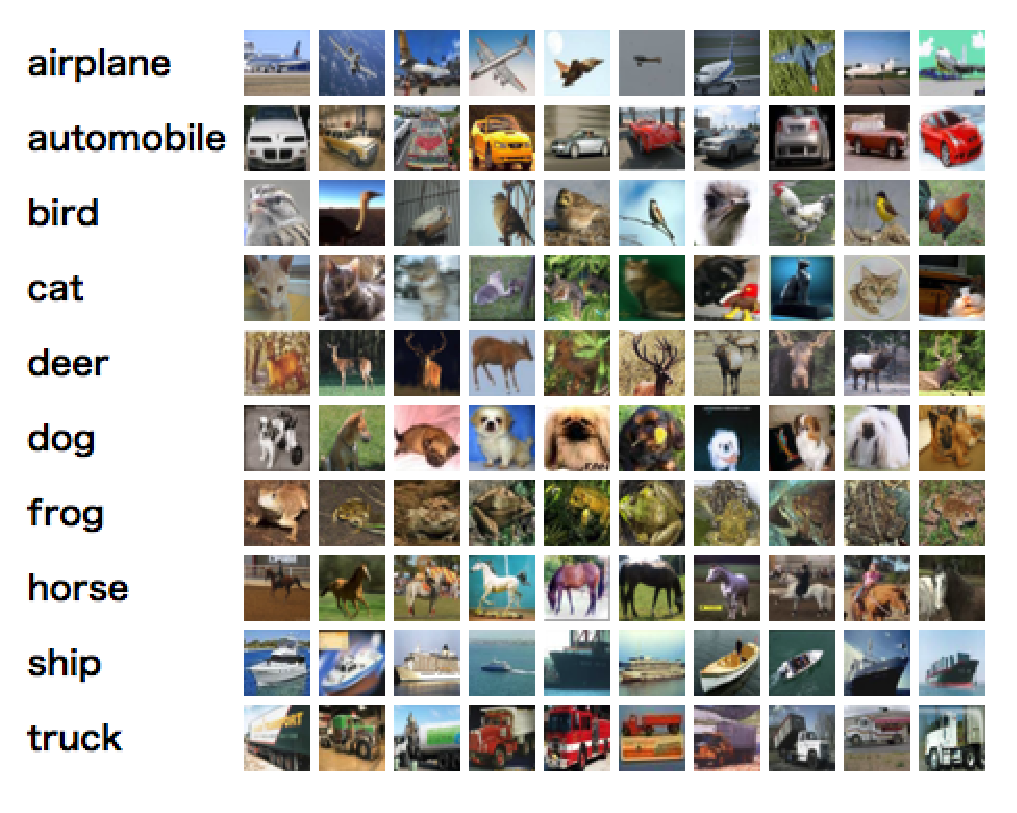
\includegraphics[width=0.8\linewidth] {images/YamasakiLab/sec2/cifar10.eps}
		\caption{CIFAR-10データセット}
		\label{fig:cifar-10}
	\end{center}
\end{figure}
\begin{practice}
dataset.pyを埋めることで,cifar10の画像を読み込むコードを完成させよ.CIFAR-10の画像はmini\_cifar/train/にある.
\end{practice}

dataset.pyを正しく書くことで以下のコマンドでCIFAR-10が実行できるようになる.
\begin{lstlisting}[basicstyle=\ttfamily\footnotesize, frame=single]
python train_cifar10_cnn.py -g 0
\end{lstlisting}
このプログラムは,mnistのプログラムとは異なり,1epochごとにmodelが出力させる.
\begin{practice}
出力されたmodelから最も精度が良いモデルを選び,そのmodelを用いて,test\_cifar10\_cnn.pyを実行せよ.
以下のコマンドでtest\_cifar10\_cnn.pyを実行できる.
\begin{lstlisting}[basicstyle=\ttfamily\footnotesize, frame=single]
python test_cifar10_cnn.py -g 0 -m (path to your model)
\end{lstlisting}
\end{practice}

\begin{practice}
(発展課題)本ネットワークの精度は約$30\sim 40$パーセントとあまり良くない.精度を上げてみよ.例えば,ネットワーク構造や,最適化手法などを変化させて見ると良い.
\end{practice}

%!TEX root = ../main.tex



\section{CNN応用分野}
これより先はCNNの応用分野であり,必須課題ではない.
画像分類以外にどのような方法でCNNが利用されているかをいくつか述べるものである.

\subsection{深層特徴}
第二章では最終層にsoftmax関数をかけてクラスの確率分布を出力していた.
CNN は最終層以外の中間層の出力も有用である.
例えば以下のVGGと呼ばれるCNNではFC6層,FC7層の値を利用することが頻繁にある.

CNNは特徴抽出と分類/回帰を同時に行うモデルである.分類/回帰の結果は最終層に現れるが,特徴表現は隠れ層に出てくるとされている.
何らかの課題を学習したCNNは,データのより良い表現(特徴)の表現を隠れ層で学習している.そのため,データの良い特徴を得るという目的で「学習済みのCNN」にデータを通しその際の隠れ層の出力を取得する,ということがよく行われる.


\begin{itembox}[l]{CNNの特徴抽出}
より正確には,CNNは最終的なタスク(分類/回帰)を行なうのに有用な特徴表現を学習する.
例えばある画像を入力に「人物が写っているか/写っていないか」の2値分類をCNNで解く場合,
恐らくCNNはそこに鳥がいるか空が写っているかなどの情報は無視して,人間の存在を分けるような特徴の表現を学習するだろう.
\end{itembox}


\subsubsection{深層特徴の利用方法}
単純に分類問題や回帰問題を解く場合は,end-to-endなネットワークを構築して学習した方が精度が高い.
しかし,ネットワーク上に問題を落とし込めない時,深層特徴だけを利用するケースがある.
例えば,画像検索などがその良い例である.
ある画像と似た画像を探したい.単純に考えると,他の画像とのピクセルレベルでの距離を計算し,近いものから取得してくるという方法が挙げられる.しかしこれには2つの問題がついてくる.それは

\begin{itemize}
	\item ピクセルレベルの距離が近いものが欲しい画像とは限らない
	\item 検索に時間がかかる
\end{itemize}

例えば左上に赤いリンゴが移った図のような写真を入力にして,他のリンゴ画像を得ようとする.しかし,図とのピクセルレベルでの距離は同じリンゴが写っているにも関わらずピクセルレベルの値の距離は大きい.これはリンゴが写っている位置が異なるために生じてしまう.また,この画像が仮に幅640px,高さ480pxだとすると$640 \times 480 = 307,200$の距離計算を行なう必要がある.

そこで,深層特徴を用いることで画像をより小さいサイズでより高次元の情報を保持した特徴に変換することで検索性能を高めることができる.先程述べた通り深層特徴は中間層の出力であり,よく用いられるネットワーク(VGG,AlexNet.ResNetなど)ではおよそ1,024-4,096次元程度のコンパクトなベクトルを得ることが出来る.
また深層特徴は(ネットワークを訓練したタスクによるが)単純なRGBではない高度な情報を保持する.この画像にどのようなものが写っているか,のような情報である.これにより色が似ているといった単純な情報以外を利用した検索が可能になる.


\subsubsection{深層特徴の抽出方法}
単純にネットワークを組んでデータを入れて中間層の値を得たとしてもそれは有用な情報ではない.
ネットワークのパラメータがデタラメなため何の意味もない値が出てくるだけである.
有用な深層特徴を得ようと思ったら,CNNを訓練しておく必要がある.

訓練の仕方は様々である.一般的には「深層特徴を利用するケースとなるべく近い形でDNNを訓練する」というのが基本である.
例えば先程の「リンゴ画像を検索したい」という例では「リンゴが写っているか否か」のDNNを訓練しその中間層を利用するという手がある.しかし普通はもう少し幅の広い課題を解くことが多く,またDNNの訓練に必要な大規模データも手に入ることは少ない.
そこでImageNetというデータセットを利用して,ImageNetデータセットの分類問題を学習したDNNの中間層出力を深層特徴として利用することが多い.
ImageNetは大量の画像を「人」「車」「鳥」のようなそこに写っているもので分類したデータセットのことであり,このデータセットで訓練したDNNモデルは他の領域にも応用しやすい汎用的な特徴表現能力を得ることが知られている.

そのため,「取り敢えず深層特徴を使いたい!」という場合は有名なネットワークをImageNetで訓練してその中間層出力を利用するケースがほとんどである.


次の章で実際に深層特徴を用いて画像検索を行なう例を見てみる.


\subsubsection{深層特徴抽出の実装}
長々書いてきたが要は深層特徴とは「データから抽出したいい感じの特徴」であり,非常に有用なものである.そのためChainerでは深層特徴を非常に簡単に得る事ができるように設計されている.


{\bf 実装課題}\\
search.pyとcreate\_db.pyを使用します
   \begin{practice}
    search.pyのargparse部分をよく読んでcifar10/test/以下から適当に画像を選んでsearch.pyをCPU上で実行せよ。
   \end{practice}
   \begin{practice}
   search.pyの中で深層特徴(src\_df)を計算する部分を探し,深層特徴のshapeを表示せよ.
   \end{practice}
   \begin{practice}
    create\_db.pyの中で深層特徴として使用する隠れ層を指定している部分を探し,VGG16のfc6層を利用するよう書き換えよ.その後もう一度search.pyを実行せよ.
   \end{practice}
   \begin{practice}
    MNISTでMLPを訓練し,その隠れ層出力を深層特徴として利用した場合の検索結果を表示せよ
    かなり難易度は高いのでTAを利用してください.
   \end{practice}


\subsection{GAN}
詳細は触れないがCNNは分類/回帰以外にも利用可能である.一例として画像生成技術であるGenerative Adversarial Network,通称GANを挙げる.
GANはgeneratorとdiscriminatorという2つのCNNを用いる.generatorは何らかの適当な入力から1枚の画像を生成するCNNである.
discriminatorは入力された画像がgeneratorが作ったものか実際の画像かを判定するCNNである.
訓練の最初の方ではgeneratorはわけの分からない画像を出力する.しかしdiscriminatorもあまり賢くないのでgeneratorの画像と実際の画像を見分けることが出来ない.その後,訓練が進むとdiscriminatorも賢くなり,generatorから出てきた画像を見抜けるようになる.そこで,generatorの損失関数をうまく設定することで,generatorはdiscriminatorを騙せるような画像を生成させるように訓練する.

generatorはdiscriminatorを騙せるような画像を生成しようとし,discriminatorはgeneratorから出てきた画像を見抜こうとする.お互いがお互いを刺激しあって学習することでgeneratorはより本物っぽい画像を生成することが出来る様になる.

Deep Convolutional GAN (通称DCGAN) の実装はchainer/examples/dcganの中にある.
generatorとdiscriminatorの定義を見つけてみよう.
また,このコードではupdaterを自作している.updaterはバッチを受け取ってモデルに通し,損失を計算してモデルの更新を行なうよう支持する場所である.
updaterはStandardUpdaterを継承してupdate\_core関数を上書きして作るのだが,もし特殊な学習を行いたければここを参考にすると良い.

\subsection{Super Resolution}
画像生成とは微妙に異なるが,CNNを利用して低画質の画像を高画質に変換しようとするものもある.
低画質の画像にはない情報を推測するのでもちろん正確な高画質画像を作ることは不可能だが,GANと組み合わせて利用するといかにも高画質画像に見える画像を生成することが出来る.

\titleformat{\chapter}[block]
{}{}{0pt}{
	\fontsize{40pt}{40pt}\selectfont\filleft
}[
\hrule 
]

% 参考文献
\bibliographystyle{plain}
\bibliography{papers}

% 追記 --------------------------------------------
\titleformat{\chapter}[block]
{}{}{0pt}{
	\fontsize{30pt}{30pt}\selectfont\filleft
}[
\hrule 
]

\titleformat{\section}[block]
{}{}{0pt}
{
	\hspace{0pt}
%	\normalfont \LARGE\bfseries \thesection
    \normalfont \LARGE\bfseries 
	\hspace{0pt}
}
[
\begin{picture}(100,0)
%\put(3,30){\color{teal}\line(1,0){400}}
\put(3,18){\color{teal}\line(1,0){350}}
\end{picture}
\\
\vspace{-50pt}
]
%!TEX root = ../main.tex

\section{謝辞}
本実験はMicrosoftの支援のもと,Microsoft Azureを使用して行われた.
Azureサーバの構築等は付録を参照のこと.

%\chapter*{付録:Azureサーバ}
%%!TEX root = ../main.tex

\setcounter{section}{0}

\parindent = 0pt

\section*{Deep Learning用VM (Linux)構築手順}
1. \url{http://portal.azure.com/}にアクセスして,マイクロソフトアカウントの{\bf[ユーザー名]}と{\bf[パスワード]}を入力して{\bf[サインイン]}をクリックする.

\begin{figure}[ht]
	\begin{center}
		\includegraphics[height=6cm]
		{images/YamasakiLab/azure/pic01.eps}
	\end{center}
\end{figure}



% -----------------------------------------------

\end{document}
